\pdfminorversion=7
\documentclass[preprint,12pt]{elsarticle}

\usepackage[T1]{fontenc}
\usepackage[utf8]{inputenc}
\usepackage{lmodern}
\usepackage{amssymb}
\usepackage{amsmath}
\usepackage{booktabs}
\usepackage{array}
\usepackage{graphicx}
\usepackage[colorlinks=true,linkcolor=blue,citecolor=blue,urlcolor=blue]{hyperref}
\hypersetup{pdfauthor={Xinchen Geng}}

\biboptions{numbers}

\setlength{\emergencystretch}{2em}
\makeatletter
\setlength{\@fptop}{0pt}
\setlength{\@fpsep}{14pt}
\setlength{\@fpbot}{0pt plus 1fil}
\makeatother
\renewcommand{\topfraction}{0.95}
\renewcommand{\bottomfraction}{0.95}
\renewcommand{\textfraction}{0.06}
\renewcommand{\floatpagefraction}{0.80}

\journal{Information Sciences}

\begin{document}

\begin{frontmatter}

\title{Causal WeatherGraph: screen--confirm--replicate discovery of lagged wind--humidity--cloud dependencies in global atmospheric reanalysis}

\author[usc]{Xinchen Geng\corref{cor1}}
\ead{gengx@usc.edu}
\cortext[cor1]{Corresponding author.}
\affiliation[usc]{organization={University of Southern California},
            city={Los Angeles},
            state={CA},
            country={USA}}

\begin{abstract}
Lagged dependency graphs mined from long, autocorrelated spatio-temporal records are easily inflated by shared history, spatial background and miscalibrated tests. We present Causal WeatherGraph, which screens physics-guided candidate edges with own-history regressions, confirms them in a dense vector autoregression conditioned on all regional histories, and replicates confirmed edges in held-out years with heteroskedasticity- and autocorrelation-consistent inference. Applied to 6-hourly ERA5 reanalysis for 1979--2025 aggregated into 66 regions, the screen retains 2,187 of 2,574 edge--lag hypotheses in 1979--2018, full conditioning confirms 1,550, and 760 replicate with the same sign in 2019--2023 and 667 in 2023--2025, against 95 and 80 of 1,024 unconfirmed hypotheses. In known-structure simulations, own-history screening recovers every true edge with precision below 0.1 under strong autocorrelation, whereas full conditioning restores F1 of 0.97--0.99 when common drivers are observed. Humidity$\rightarrow$cloud dependence is modestly stronger than its reverse, also with CERES satellite cloud in 2017--2023, whereas wind--humidity dependence has no consistent direction. A pre-specified wind--humidity eddy convergence, the quadratic term of an exact moisture-flux decomposition, reduces held-out midlatitude cloud-prediction error by 0.36--0.46\%, 2.5--3.1 times the tropical gain, whereas remote and time-shifted versions add nothing. Physics-guided edges exceed distance-matched random edges by only 4 percentage points in significance rate, chain counts are not enriched, summed path lags of about 24~h follow the lag window, seasonal modulation reverses sign between hemispheres, and cloud-state contrasts do not replicate. Wind--cloud dependence largely persists after conditioning on intermediate humidity. The recovered structure consists of distributed, conditional linear predictive dependencies rather than interventional effects.
\end{abstract}

\begin{highlights}
\item Screen--confirm--replicate framework for lagged dependency graphs in reanalysis
\item Eddy wind--humidity convergence improves held-out midlatitude cloud prediction
\item Confirmed edges replicate at 49\% and 43\% in two held-out periods, controls 8--9\%
\item Humidity-to-cloud exceeds its reverse; CERES cloud confirms it for 2017--2023
\item No support for chain enrichment, uniform winter strengthening or cloud regimes
\end{highlights}

\begin{keyword}
lagged dependency discovery \sep Granger causality \sep spatio-temporal data mining \sep replicability \sep vector autoregression \sep atmospheric reanalysis
\end{keyword}

\end{frontmatter}

\section{Introduction}
\label{sec:intro}

Wind, humidity and cloud are coupled through transport, thermodynamics and phase change. Synoptic circulation organizes the transport of moisture in extratropical cyclones, whose warm conveyor belts lift moist air into cloud and precipitation \citep{Heitmann2024WCB}; storm-track intensity differs between the hemispheres with topography and ocean energy transport \citep{Shaw2022Stormier}; and cloud responds to large-scale cloud-controlling factors that include humidity, vertical motion and stability \citep{Andersen2023CloudSensitivities}. For such a coupled system, forecast skill alone does not reveal how variables depend on one another across regions and time lags, which dependencies recur across decades and atmospheric states, or which apparent pathways are artefacts of how the data were sampled and analysed. Long global reanalysis records make these questions empirically approachable, provided that the discovery procedure can separate replicable structure from the many spurious dependencies that strongly autocorrelated spatio-temporal data generate.

Three lines of research bear on this problem. Global data-driven forecasting systems such as GraphCast \citep{Lam2023GraphCast}, Pangu-Weather \citep{Bi2023Pangu}, NeuralGCM \citep{Kochkov2024NeuralGCM} and GenCast \citep{Price2025GenCast} now rival operational numerical prediction, and WeatherBench~2 standardizes their evaluation \citep{Rasp2024WeatherBench2}. Spatio-temporal graph learning infers or updates adjacency from data, including hierarchical station--variable graphs for weather \citep{Ma2023HiSTGNN} and evolving graph structures for multivariate series \citep{Ye2025EvolvingGraph}. Causal discovery for time series tests directed lagged dependence through temporal precedence \citep{Shojaie2022Granger} and, in the Earth sciences, through conditional-independence testing combined with domain knowledge \citep{Runge2023TimeSeries}, with PCMCI \citep{Runge2019PCMCI}, regime-dependent extensions \citep{Saggioro2020RegimePCMCI} and space--time stencil methods for gridded data \citep{Nichol2025CaStLe} as prominent examples.

None of these strands directly delivers replicable directed dependencies from global reanalysis. The weights and learned adjacencies of forecasting models are optimized for predictive skill and need not represent directed dependence. Causal-discovery methods, in turn, meet unusually adverse data. Reanalysis fields are inferences from data assimilation with a forecast model rather than direct observations, and in ERA5 total cloud cover is a model diagnostic constrained only indirectly by the assimilated observations \citep{Soci2024ERA5}, so that it inherits biases of the model's cloud physics \citep{Hellmuth2025CloudPhase}. Strong autocorrelation, diurnal and seasonal cycles, spatial smoothing and shared synoptic forcing further inflate nominal significance \citep{Runge2023TimeSeries}. A single-stage screen that conditions only on each target's own history illustrates the problem: applied to 47 years of ERA5, it declares 14,308 of 18,018 edge--lag--regime tests significant, a nearly saturated graph whose orientation is partly fixed by the candidate list. We therefore ask the following question: which lagged dependencies among wind, humidity and cloud in long-term global reanalysis survive conditioning on all observed regional histories and replicate in held-out years, and which apparent pathway properties are artefacts of the discovery design? Our primary objective is to identify this replicable set of conditional lagged dependencies. Our secondary objectives are to quantify how much of the screened structure reflects spatial background, imposed orientation, endogenous regime selection and the tested lag window, to check whether the humidity--cloud dependence persists when reanalysis cloud is replaced by an independent satellite product, and to test with a pre-specified index whether the quadratic wind--humidity part of the moisture flux carries information about cloud that linear models of regional anomalies miss.

We propose Causal WeatherGraph, a framework that turns this question into a three-stage discovery procedure (Figure~\ref{fig:framework}). The framework aggregates gridded fields into regional anomaly series whose preprocessing is fitted only on a discovery period, restricts the hypothesis space with physics-guided candidate edges, and then (i) screens candidates with an own-history nested regression, which favours recall; (ii) confirms screened candidates in a dense vector autoregression that conditions on every observed regional history, which favours precision; and (iii) replicates confirmed candidates in held-out years with directional tests and frozen-coefficient predictive gains, using unconfirmed candidates as a negative control. All tests use calendar-time heteroskedasticity- and autocorrelation-consistent (HAC) inference \citep{Lazarus2021HAR}. A validation suite surrounds the three stages: known-null and known-structure simulations, distance-matched null graphs, symmetric direction tests, direct regime-interaction tests, moisture-transport diagnostics, a pre-specified wind--humidity eddy convergence test and an independent satellite cloud product. Throughout, the term ``causal'' in the framework name refers to Granger-type lagged predictive dependence given a stated information set; it does not denote an interventional effect.

\begin{figure}[htbp]
\centering
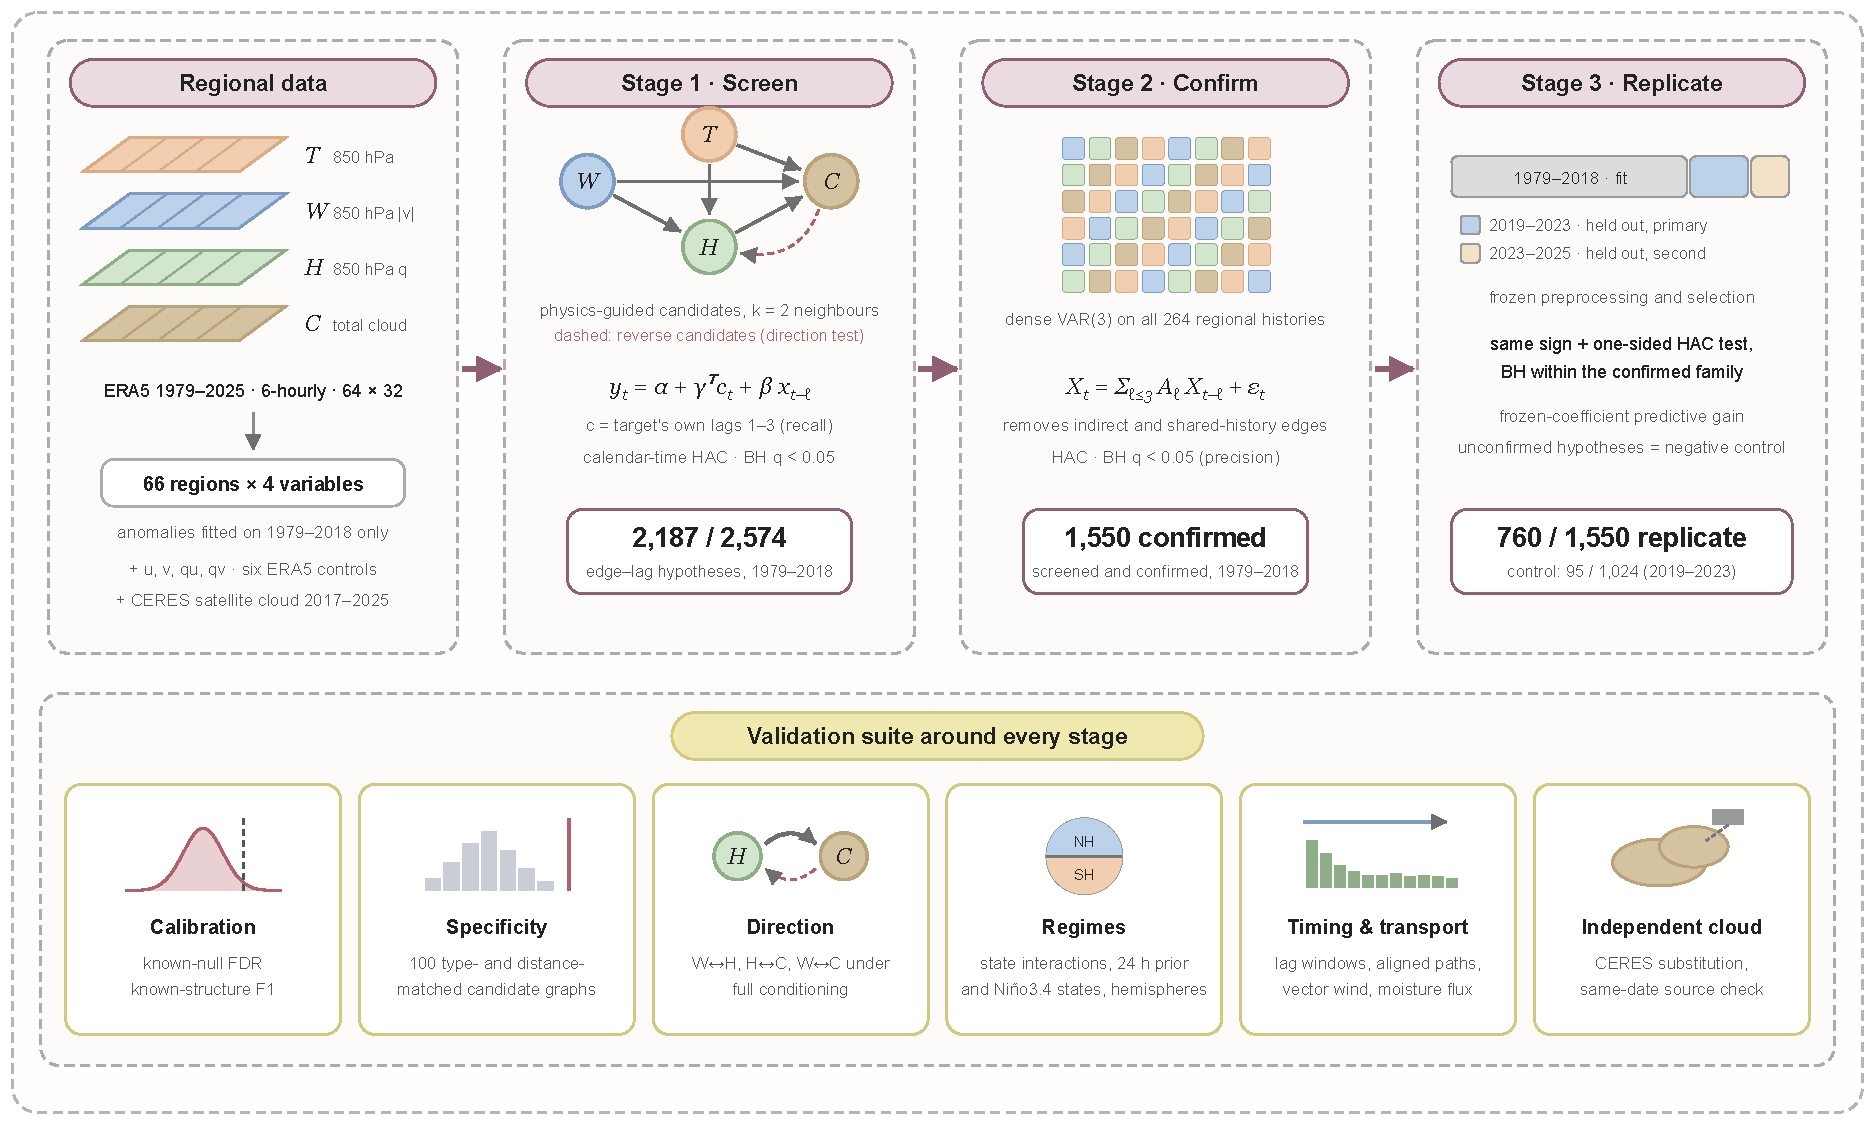
\includegraphics[width=0.98\textwidth]{figures/fig01_framework.pdf}
\caption{Overview of Causal WeatherGraph. Physics-guided candidates are screened with own-history regressions, confirmed under full conditioning and replicated in held-out years, while a validation suite tests calibration, specificity, direction, regime dependence, timing and product dependence.}
\label{fig:framework}
\end{figure}

We make four main contributions:
\begin{itemize}
\item \textbf{A screen--confirm--replicate framework.} We separate recall-oriented screening of physics-guided candidates, confirmation under full conditioning on all observed regional histories, and held-out replication with a negative control, so that replicable dependencies are distinguished from shared-history, indirect and spatial-background artefacts in large spatio-temporal records.
\item \textbf{Calibration and benchmarking.} We calibrate each stage with known-null and known-structure simulations and compare it with multivariable Granger regression, PCMCI, Regime-PCMCI and CaStLe under matched information, together with runtime and memory measurements, showing that single-stage own-history screening is reliable only for weakly coupled systems.
\item \textbf{A replicable wind--humidity--cloud dependency set.} We apply the framework to 47 years of ERA5 and to CERES satellite cloud, identify 760 replicated conditional dependencies, and show which pathway properties survive, notably a modest humidity$\rightarrow$cloud asymmetry, and which do not, namely chain enrichment, window-free interpretation of path lags, uniform winter strengthening and cloud-state regimes.
\item \textbf{A pre-specified eddy predictor of cloud.} We decompose the 850-hPa moisture flux exactly into climatological, linear and quadratic parts, define a regional wind--humidity eddy convergence (WHEC) from the quadratic part, and show in a test frozen before any result that it reduces held-out cloud-prediction error beyond the dense autoregression and linear transport terms, with midlatitude gains 2.5--3.1 times the tropical gains, whereas remote-region and time-shifted versions add nothing.
\end{itemize}

\section{Related Work}
\label{sec:related}

\subsection{Data-driven atmospheric prediction and learned graphs}

Global data-driven forecasting has progressed from neural operators and three-dimensional networks to graph-based, hybrid and probabilistic systems. GraphCast \citep{Lam2023GraphCast} and Pangu-Weather \citep{Bi2023Pangu} established medium-range skill comparable with operational systems, NeuralGCM couples learned components with a differentiable dynamical core \citep{Kochkov2024NeuralGCM}, and GenCast generates probabilistic ensembles \citep{Price2025GenCast}. Spatio-temporal graph neural networks learn adjacency jointly with forecasts, for example hierarchical graphs that link station-level and variable-level structure for weather prediction \citep{Ma2023HiSTGNN} and evolving graph structures for multivariate series \citep{Ye2025EvolvingGraph}, whereas carefully specified linear models remain strong multivariate forecasting baselines \citep{Zeng2023DLinear}. These models minimize predictive loss. Their attention weights and learned adjacencies are not tested hypotheses about directed lagged dependence, and none of them controls or verifies the error rate of the structure it implies.

\subsection{Causal discovery for Earth-system time series}

Granger's criterion asks whether the history of a source improves the prediction of a target given a stated information set; its multivariable form conditions on all observed histories in a vector autoregression, and recent extensions address high-dimensional, nonlinear and subsampled series \citep{Shojaie2022Granger}. Earth-system applications combine this idea with conditional-independence testing and domain knowledge \citep{Runge2023TimeSeries}, and causal-network analyses of teleconnections state the assumed pathways and information sets explicitly before quantifying them \citep{Kretschmer2021Pathways}. PCMCI selects conditioning sets with a PC-type stage before testing momentary conditional independence and was designed for large nonlinear systems \citep{Runge2019PCMCI}. Neural methods address irregular sampling \citep{Cheng2023CUTS} and history-dependent noise \citep{Gong2023Rhino}, structure learning has been extended to high-dimensional non-stationary series \citep{Chen2024NonstationaryCausal}, and background knowledge can be requested dynamically to constrain the search \citep{Kitson2025RequestedKnowledge}. Comparisons on synthetic systems and climate indices show that causal methods outperform correlation analysis but can disagree with one another \citep{Docquier2024Comparison}, and benchmarks generated from real series with known graphs have been proposed to evaluate such methods \citep{Cheng2024CausalTime}. Two approaches are closest to our setting. Regime-PCMCI learns persistent hidden regimes jointly with regime-specific causal graphs \citep{Saggioro2020RegimePCMCI}, and CaStLe exploits local space--time stencils and spatial homogeneity to discover structure on gridded fields \citep{Nichol2025CaStLe}. Both target identification under explicit assumptions on comparatively small or spatially homogeneous systems. Neither is designed to verify whether a large, nearly saturated discovered graph replicates out of sample, which is the gap that our framework addresses (Table~\ref{tab:positioning}).

\begin{table}[htbp]
\centering
\caption{Positioning of Causal WeatherGraph relative to related approaches.}
\label{tab:positioning}
\footnotesize
\setlength{\tabcolsep}{3pt}
\begin{tabular}{@{}p{0.16\textwidth}p{0.17\textwidth}p{0.17\textwidth}p{0.20\textwidth}p{0.235\textwidth}@{}}
\toprule
Approach & Candidate space & Conditioning & Regimes and space & Verification of the graph \\
\midrule
Multivariable Granger \citep{Shojaie2022Granger} & All pairs & All observed lags & None & In-sample tests \\
PCMCI \citep{Runge2019PCMCI} & All pairs or assumed links & PC-selected parents & None & In-sample tests \\
Regime-PCMCI \citep{Saggioro2020RegimePCMCI} & All pairs or assumed links & PC-selected parents per regime & Learned hidden persistent regimes & In-sample tests \\
CaStLe \citep{Nichol2025CaStLe} & Local stencil neighbours & Stencil parents & Shared local stencil on a grid & In-sample tests \\
Causal WeatherGraph (this work) & Physics-guided set plus symmetric reverse set & Own history (screen); all 264 regional histories (confirm) & Prescribed, antecedent and external states with interaction tests; distance-matched null graphs & Held-out replication, frozen predictive gain, negative control, satellite substitution \\
\bottomrule
\end{tabular}
\end{table}

\subsection{Atmospheric regimes, cloud-controlling factors and reanalysis}

Extratropical clouds are organized by the large-scale circulation and hydrological cycle; across climate models, the sensitivity of Southern Ocean cloud liquid water to moisture convergence helps predict the shortwave cloud feedback \citep{McCoy2022Extratropical}. Cloud-controlling-factor analyses relate cloud and cloud-radiative anomalies to large-scale humidity, stability, vertical motion and advection, for example with regularized regressions fitted to two decades of near-global satellite and reanalysis data \citep{Andersen2023CloudSensitivities}, and a systematic evaluation extends this approach to high clouds and shows that thermodynamic structure above the boundary layer is an important controlling factor \citep{WilsonKemsley2024HighCloud}. Moisture budgets separate the convergence by the time-mean flow from that by eddies; in the Mediterranean, for example, an ERA5 budget attributes the convergence of ocean-derived moisture over land mainly to submonthly transient eddies \citep{Tootoonchi2025Mediterranean}. These studies motivate our variables, transport diagnostics and eddy predictor, but they are predominantly contemporaneous or climatological, whereas we target lagged, region-to-region dependence at six-hourly resolution. Reanalysis adds a further layer of caution: ERA5 merges observations with a forecast model, so its fields inherit model physics, assimilation increments and spatial smoothing \citep{Soci2024ERA5}, and its cloud fields inherit biases of the cloud microphysics, such as an overestimated frequency of supercooled liquid-containing clouds at mid and high latitudes relative to CloudSat--CALIPSO \citep{Hellmuth2025CloudPhase}. We therefore treat dependencies in ERA5 as properties of the reanalysis product and test the humidity--cloud dependence against an independent satellite retrieval.

\section{Methodology}
\label{sec:method}

\subsection{Problem formulation and estimands}

Let
\begin{equation}
\mathcal{X}^{\mathrm{raw}}=\left\{x^{\mathrm{raw}}_{t,n,v}\right\}\in\mathbb{R}^{N_t\times N\times V}
\end{equation}
denote a multivariate atmospheric field observed at time $t\in\{1,\ldots,N_t\}$, grid node $n\in\{1,\ldots,N\}$ and variable $v\in\mathcal{V}$, with $N_t=68{,}668$ six-hourly times, $N=2{,}048$ grid nodes and
\begin{equation}
\mathcal{V}=\{T,\,H,\,W,\,C\},\qquad V=4,
\end{equation}
where $T$ is temperature, $H$ specific humidity, $W$ wind speed and $C$ total cloud cover. Spatial aggregation (Section~\ref{subsec:anom}) yields regional anomaly series $X_{t,r,v}$ for regions $r\in\mathcal{R}$, $|\mathcal{R}|=66$, so that $\mathbf{X}_t\in\mathbb{R}^{264}$.

For a candidate edge $e:(i,a)\rightarrow(j,b)$ and a lag $\ell$, the estimand is the coefficient of $X_{t-\ell,i,a}$ in the linear projection of $X_{t,j,b}$ on an information set $\mathcal{I}_t$,
\begin{equation}
\beta_{e,\ell}(\mathcal{I})=\text{coefficient of }X_{t-\ell,i,a}\text{ in }\mathrm{Proj}\left(X_{t,j,b}\,\middle|\,\mathcal{I}_t\cup\{X_{t-\ell,i,a}\}\right),
\label{eq:estimand}
\end{equation}
and the edge--lag hypothesis is $H_0^{(e,\ell)}:\beta_{e,\ell}(\mathcal{I})=0$. We use two information sets: the own-history set $\mathcal{I}^{\mathrm{own}}_t=\{X_{t-k,j,b}\}_{k=1}^{3}$ and the full set $\mathcal{I}^{\mathrm{full}}_t=\{\mathbf{X}_{t-k}\}_{k=1}^{3}$ of all 264 regional histories. A nonzero $\beta_{e,\ell}(\mathcal{I})$ means that the source lag improves linear prediction of the target given $\mathcal{I}$; it does not identify the effect of intervening on the source.

We use the following counting units consistently. A \emph{candidate edge} is a directed region--variable pair; an \emph{edge--lag hypothesis} is a candidate edge at one lag; an \emph{edge--lag--regime test} is one hypothesis evaluated in one regime; a \emph{unique edge} collapses significant hypotheses over lags; and a \emph{lag-resolved chain} is a two-step path with specified lags. Every fraction reported below states its denominator in one of these units.

\subsection{Data, variables and acquisition routes}
\label{subsec:data}

We use the ERA5 global reanalysis \citep{Soci2024ERA5} at 6-hourly resolution from 1979-01-01 00 UTC to 2025-12-31 18 UTC on a $64\times32$ regular latitude--longitude grid. For 1979-01-01 to 2023-01-10 we use the WeatherBench~2 product \citep{Rasp2024WeatherBench2}, which regrids ERA5 conservatively from its native resolution; for 2023-01-11 to 2025-12-31, where that product ends, we retrieve the native $0.25^\circ$ fields from the Copernicus Climate Data Store (CDS) and regrid them to the same grid with the same first-order conservative scheme. The aligned record has 68,668 timestamps with no missing or duplicated times, and nonfinite values stop the pipeline rather than being interpolated.

Temperature, specific humidity and the horizontal wind components $u$ and $v$ are taken at 850~hPa, and total cloud cover is a single-level field. The 850-hPa level samples the lower free troposphere above most of the boundary layer, where extratropical cyclones carry the moist air that their warm conveyor belts lift into cloud \citep{Heitmann2024WCB}. Scalar wind speed $W=(u^2+v^2)^{1/2}$ measures circulation intensity irrespective of direction; because it carries no transport direction, we evaluate direction separately with along-connection wind and moisture-flux projections (Section~\ref{subsec:paths}). Total cloud cover integrates cloud over model levels and is the quantity most directly comparable with satellite cloud-area retrievals. The variables therefore have different vertical supports, and the 850-hPa level lies below the surface in some high-terrain cells.

Three caveats specific to reanalysis shape our design. First, ERA5 total cloud cover is a model diagnostic that depends on the model's humidity and cloud scheme, so a humidity$\rightarrow$cloud dependence could partly be built into the product; we test this with CERES SYN1deg Edition~4.2 hourly satellite cloud area for 2017--2025, retrieved with the CERES Edition~4 cloud algorithms \citep{Minnis2021CERES}. Second, assimilation and conservative regridding smooth the fields and induce spatial dependence among neighbouring regions, which we address with distance-matched null graphs. Third, the record joins two sources, and the regridding route matters. Fields requested directly on the coarse CDS grid are interpolated rather than area-averaged: on 152 identical timestamps in 2022 and January 2023 they give wind speeds 0.69~m\,s$^{-1}$ higher than WeatherBench~2, a level shift of 0.20 discovery standard deviations in the regional wind series, and regional anomaly correlations of only 0.907--0.991 (Supplementary Table~S1). Native fields regridded conservatively reproduce WeatherBench~2 on the same timestamps, with regional anomaly differences below $3\times10^{-5}$ discovery standard deviations and correlations of 1.000, so the record is homogeneous across the splice. We keep the 2019-01-01 to 2023-01-10 segment, specified before the re-acquisition, as the primary replication segment and use 2023-01-11 to 2025-12-31 as a second replication segment.

We also use $u$, $v$ and the grid-cell products $qu$ and $qv$ for transport diagnostics; six ERA5 control fields (vertical pressure velocity at 500 and 700~hPa, 500-hPa geopotential, 700-hPa temperature, surface pressure and mean sea-level pressure) for physical-control sensitivity analyses; and the monthly Ni\~no-3.4 index for externally defined states. Table~\ref{tab:data} summarizes the configuration.

\begin{table}[htbp]
\centering
\caption{Data and main configuration.}
\label{tab:data}
\footnotesize
\begin{tabular}{@{}p{0.30\textwidth}p{0.64\textwidth}@{}}
\toprule
Item & Setting \\
\midrule
Record & ERA5, 1979-01-01 00 UTC to 2025-12-31 18 UTC, 6-hourly, 68,668 times \\
Sources & WeatherBench~2 to 2023-01-10; native CDS fields with the same conservative regridding afterwards \\
Grid and regions & $64\times32$ grid (2,048 nodes); $6\times11$ latitude--longitude bins, 66 regions \\
Variables & 850-hPa temperature, specific humidity and wind speed; total cloud cover \\
Additional data & $u$, $v$, $qu$, $qv$ and eddy-convergence indices; six ERA5 controls; Ni\~no-3.4; CERES SYN1deg Ed4.2 hourly cloud area (2017--2025) \\
Temporal split & Discovery 1979--2018 (58,437 responses); held-out 2019-01-01 to 2023-01-10 (5,884, primary) and 2023-01-11 to 2025-12-31 (4,344, second replication) \\
Preprocessing & Cell-wise monthly climatology and standardization fitted on 1979--2018 only \\
Candidates & $k=2$ nearest neighbours; 858 candidates, 2,574 edge--lag hypotheses (lags 1--3, 6--18~h); symmetric set 1,272 candidates, 3,816 hypotheses \\
Stage 1 (screen) & Own-history nested regression, HAC (Bartlett, 64 steps), BH over 2,574 hypotheses \\
Stage 2 (confirm) & Dense VAR(3) on 264 regional series (793 parameters per equation), HAC, BH over 2,574 \\
Stage 3 (replicate) & Same-sign one-sided HAC test and frozen predictive gain, BH within the confirmed family \\
\bottomrule
\end{tabular}
\end{table}

\subsection{Anomaly construction and spherical regionalization}
\label{subsec:anom}

To suppress the annual cycle without leaking held-out information, we remove a calendar-month climatology and standardize every grid node and variable using the discovery period $\mathcal{D}$ (1979--2018) only:
\begin{equation}
a_{t,n,v}=x^{\mathrm{raw}}_{t,n,v}-\mu^{\mathcal{D}}_{m(t),n,v},\qquad
z_{t,n,v}=\frac{a_{t,n,v}-\bar{a}^{\mathcal{D}}_{n,v}}{\max\left(\sigma^{\mathcal{D}}_{n,v},10^{-8}\right)},
\end{equation}
where $m(t)$ is the calendar month of $t$, $\mu^{\mathcal{D}}_{m,n,v}$ is the discovery-period monthly mean, and $\bar{a}^{\mathcal{D}}_{n,v}$ and $\sigma^{\mathcal{D}}_{n,v}$ are the discovery-period anomaly mean and standard deviation. The fitted transformation is applied unchanged to 2019--2025, so no held-out observation updates any statistic. Because a monthly climatology leaves the diurnal cycle in the anomalies, we repeat the complete three-stage analysis with a calendar-month $\times$ UTC-hour climatology as a sensitivity analysis. The descriptive full-record screening in Section~\ref{subsec:regime_res} fits the climatology on 1979--2025 and is labelled accordingly.

The grid is partitioned into $n_\phi=\operatorname{round}(\sqrt{R_0/2})=6$ latitude and $n_\lambda=\lceil R_0/n_\phi\rceil=11$ longitude bins for a requested $R_0=64$, giving 66 non-empty regions. Regional series are arithmetic means of standardized grid anomalies,
\begin{equation}
X_{t,r,v}=\frac{1}{|\mathcal{R}_r|}\sum_{n\in\mathcal{R}_r}z_{t,n,v},\qquad \mathbf{X}\in\mathbb{R}^{N_t\times66\times4},
\end{equation}
regional longitudes are circular means, and inter-regional distances are great-circle distances,
\begin{align}
a_{ij}&=\sin^{2}\!\left(\tfrac{\phi_i-\phi_j}{2}\right)+\cos\phi_i\cos\phi_j\sin^{2}\!\left(\tfrac{\lambda_i-\lambda_j}{2}\right),\\
d_{ij}&=2R_{\oplus}\arcsin\sqrt{a_{ij}},\qquad R_{\oplus}=6{,}371\ \mathrm{km}.
\end{align}
Aggregation can mix distinct weather systems within a region; alternative regionalizations are reported in Supplementary Table~S5.

\subsection{Physics-guided and symmetric candidate graphs}

An unconstrained search over all region--variable pairs would require $O(R^2V^2L)$ tests and would spend most of the multiple-testing budget on physically uninformative pairs. We therefore define a candidate graph $\mathcal{G}^0=(\mathcal{U},\mathcal{E}^0)$ on region--variable nodes $\mathcal{U}=\mathcal{R}\times\mathcal{V}$ from two relation sets,
\begin{align}
\mathcal{P}_{\mathrm{local}}&=\{W\!\rightarrow\!H,\,H\!\rightarrow\!C,\,T\!\rightarrow\!H,\,T\!\rightarrow\!C,\,W\!\rightarrow\!C\},\\
\mathcal{P}_{\mathrm{spatial}}&=\{W\!\rightarrow\!H,\,H\!\rightarrow\!H,\,H\!\rightarrow\!C,\,W\!\rightarrow\!C\},
\end{align}
and the $k$ nearest source regions $\mathcal{N}_k(j)$ of each target $j$:
\begin{multline}
\mathcal{E}^{0}=\left\{(r,a)\!\rightarrow\!(r,b):(a,b)\in\mathcal{P}_{\mathrm{local}}\right\}\\
\cup\left\{(i,a)\!\rightarrow\!(j,b):i\in\mathcal{N}_{k}(j),\ (a,b)\in\mathcal{P}_{\mathrm{spatial}}\right\}.
\end{multline}
With $k=2$, $|\mathcal{E}^0|=66\times5+66\times2\times4=858$, and lags $\ell\in\{1,2,3\}$ give 2,574 edge--lag hypotheses. These restrictions focus the search on the question of interest; they do not establish physical admissibility, and they fix the orientation of the wind--humidity--cloud pathway by construction. To test orientation rather than impose it, we form a symmetric candidate set that contains, for every $W$--$H$, $H$--$C$ and $W$--$C$ pair on the union of the matched spatial supports, both directions. It has 212 candidates per direction, 1,272 in total, and 3,816 edge--lag hypotheses.

\subsection{Stage 1: own-history screening}

For a candidate $e:(i,a)\rightarrow(j,b)$ at lag $\ell$, let $y_t=X_{t,j,b}$, $x_t=X_{t-\ell,i,a}$ and $\mathbf{c}_t=[X_{t-1,j,b},X_{t-2,j,b},X_{t-3,j,b}]^{\top}$. The restricted and full models are
\begin{align}
\mathcal{M}_{R}:\quad y_t&=\alpha_R+\boldsymbol{\gamma}_R^{\top}\mathbf{c}_t+\varepsilon^{R}_t,\\
\mathcal{M}_{F}:\quad y_t&=\alpha_F+\boldsymbol{\gamma}_F^{\top}\mathbf{c}_t+\beta_{e,\ell}x_t+\varepsilon^{F}_t,
\end{align}
fitted by ordinary least squares on the set $\mathcal{J}$ of response times of the period or regime. By the Frisch--Waugh--Lovell theorem, with $\mathbf{M}_C=\mathbf{I}-\mathbf{C}(\mathbf{C}^{\top}\mathbf{C})^{-1}\mathbf{C}^{\top}$,
\begin{equation}
\widetilde{\mathbf{y}}=\mathbf{M}_C\mathbf{y},\qquad\widetilde{\mathbf{x}}=\mathbf{M}_C\mathbf{x},\qquad\widehat{\beta}_{e,\ell}=\frac{\widetilde{\mathbf{x}}^{\top}\widetilde{\mathbf{y}}}{\widetilde{\mathbf{x}}^{\top}\widetilde{\mathbf{x}}},
\end{equation}
so the restricted fit is shared by all candidate sources of the same target. Because residuals remain autocorrelated and heteroskedastic (Section~\ref{subsec:calib}), we replace the nested $F$-test with a calendar-time HAC variance with a Bartlett kernel \citep{Lazarus2021HAR},
\begin{equation}
\widehat{\mathrm{Var}}(\widehat{\beta}_{e,\ell})=\frac{n}{n-p}\,\frac{\sum_{|h|\le B}\left(1-\frac{|h|}{B+1}\right)\sum_{t}s_t s_{t-h}}{\left(\widetilde{\mathbf{x}}^{\top}\widetilde{\mathbf{x}}\right)^{2}},\qquad s_t=\widetilde{x}_t\,\widehat{\varepsilon}^{F}_t,
\label{eq:hac}
\end{equation}
where $n$ is the number of responses, $p$ the number of parameters, and $B=64$ six-hourly steps (16 days), with $B\in\{32,128\}$ as sensitivity values. Times excluded by a regime mask contribute $s_t=0$ at their original calendar positions, so separated dates are never treated as neighbours. Two-sided normal $p$-values are adjusted by the Benjamini--Hochberg (BH) procedure \citep{Benjamini1995} within an explicitly stated family,
\begin{equation}
q_{(i)}=\min\left\{1,\min_{k\ge i}\frac{M}{k}\,p_{(k)}\right\},
\end{equation}
where $p_{(1)}\le\dots\le p_{(M)}$ are the ordered $p$-values of the family. In the three-stage analysis the family is all 2,574 hypotheses; in the descriptive regime screening we report both regime $\times$ target-variable families and the global family of 18,018 tests. Effect sizes are reported as
\begin{equation}
\Delta R^2=\frac{\mathrm{RSS}_R-\mathrm{RSS}_F}{\mathrm{TSS}},\qquad
R^2_{\mathrm{partial}}=\frac{\mathrm{RSS}_R-\mathrm{RSS}_F}{\mathrm{RSS}_R}.
\end{equation}
Stage~1 is designed for recall: in known-structure simulations it detects every true edge but also indirect and common-driver dependencies (Section~\ref{subsec:calib}).

\subsection{Stage 2: confirmation in a dense vector autoregression}

Screened hypotheses are re-estimated in a dense vector autoregression of order three,
\begin{equation}
\mathbf{X}_t=\mathbf{c}+\sum_{\ell=1}^{3}\mathbf{A}_{\ell}\mathbf{X}_{t-\ell}+\boldsymbol{\varepsilon}_t,\qquad\mathbf{X}_t\in\mathbb{R}^{264},
\label{eq:var}
\end{equation}
which is the multivariable form of Granger's criterion \citep{Shojaie2022Granger}. Each equation has 793 parameters and is estimated by unpenalized least squares through one shared QR decomposition; the design is full rank, with condition number 218 in 1979--2018. For hypothesis $(e,\ell)$ the coefficient of interest is $\beta^{\mathrm{full}}_{e,\ell}=[\mathbf{A}_{\ell}]_{(j,b),(i,a)}$, whose HAC variance is computed as in Eq.~\eqref{eq:hac} from the influence scores $s_t=\mathbf{d}_t\widehat{\varepsilon}_{t,(j,b)}$, where $\mathbf{d}_t$ is the corresponding row of $\mathbf{Q}\mathbf{R}^{-\top}$. A hypothesis is \emph{confirmed} if it passes Stage~1 and its BH-adjusted $q$-value over the 2,574 hypotheses is below 0.05. Conditioning on all observed histories removes dependencies that arise only through other observed variables; it cannot remove dependencies induced by unobserved drivers.

\subsection{Stage 3: replication in held-out years}

Confirmed hypotheses are evaluated on held-out years with preprocessing, candidate selection and stage decisions frozen. The primary held-out segment is 2019-01-01 to 2023-01-10 (5,884 responses); the second, 2023-01-11 to 2025-12-31 (4,344 responses), is evaluated with the same frozen rules and reported separately. In each segment we refit Eq.~\eqref{eq:var}, allowing lags to reach into the preceding period, and compute a one-sided directional $p$-value
\begin{equation}
p^{\mathrm{rep}}_{e,\ell}=\begin{cases}p_{e,\ell}/2,&\operatorname{sign}\widehat{\beta}^{\mathrm{held}}_{e,\ell}=\operatorname{sign}\widehat{\beta}^{\mathrm{disc}}_{e,\ell},\\1-p_{e,\ell}/2,&\text{otherwise},\end{cases}
\end{equation}
where $p_{e,\ell}$ is the two-sided HAC $p$-value in the held-out segment. A confirmed hypothesis \emph{replicates} if its BH-adjusted $p^{\mathrm{rep}}$ within the confirmed family is below 0.05, a selective two-stage design in the spirit of replicability analysis \citep{Bogomolov2023Replicability}. We additionally freeze the discovery coefficients and compute the held-out predictive gain of each source lag,
\begin{equation}
G_{e,\ell}=\frac{1}{n_{\mathrm{held}}}\sum_{t\in\mathrm{held}}\left[\left(e^{R}_{t}\right)^{2}-\left(e^{F}_{t}\right)^{2}\right],
\end{equation}
where $e^{F}_t$ is the frozen full-model error and $e^{R}_t$ the error of the exact restricted refit without that coefficient, obtained by an inverse-Gram update of the discovery fit; $G_{e,\ell}$ is tested one-sidedly with a HAC standard error. Finally, we apply the same replication rule to all hypotheses that failed Stage~1 or Stage~2 as a \emph{negative control}. Because the held-out years also enter the descriptive full-record screening (Section~\ref{subsec:regime_res}), this is a retrospective temporal holdout with frozen procedures rather than a prospective test.

\subsection{Regimes, seasons and external states}
\label{subsec:regimes}

The descriptive screening uses seven regimes,
\begin{equation}
\mathcal{S}=\{\text{all},\ \text{DJF},\ \text{JJA},\ \text{high}\,H,\ \text{normal}\,H,\ \text{high}\,C,\ \text{normal}\,C\}.
\end{equation}
Humidity and cloud states are defined from spatially averaged regional indices $g^{H}_t=R^{-1}\sum_r X_{t,r,H}$ and $g^{C}_t=R^{-1}\sum_r X_{t,r,C}$, with high states $g_t\ge Q_{0.8}(g)$, normal humidity $Q_{0.2}(g^H)<g^H_t<Q_{0.8}(g^H)$, normal cloud $g^C_t<Q_{0.8}(g^C)$, and the mask applied at the response time $t$. Because $g^{C}_t$ contains the response itself, such masks select on the outcome and can distort regime contrasts. We therefore (i) refit the thresholds on 1979--2018; (ii) define antecedent states from $g_{t-4}$, which precede every tested source lag; (iii) define external states from the Ni\~no-3.4 anomaly of the last complete month before the earliest source, with thresholds of $\pm0.66\,^{\circ}$C fitted on the 480 discovery months; and (iv) test regime differences directly with the interaction model
\begin{equation}
y_t=\alpha_{s(t)}+\boldsymbol{\gamma}_{s(t)}^{\top}\mathbf{c}_t+\beta x_t+\delta\,x_t\,\mathbb{I}[s(t)=\mathrm{high}]+\varepsilon_t,
\end{equation}
with state-specific intercepts and own-history coefficients and a HAC test of $\delta=0$, rather than comparing separately selected graphs. Seasons are defined locally: winter is DJF in the Northern Hemisphere (NH) and JJA in the Southern Hemisphere (SH). For 425 candidate pairs whose source and target regions mirror each other across the equator, we estimate the signed local winter-minus-summer slope difference $\Delta=\beta_{\mathrm{winter}}-\beta_{\mathrm{summer}}$ in each hemisphere and the contrast $\Delta_{\mathrm{NH}}-\Delta_{\mathrm{SH}}$, combining the influence scores of both hemispheres on the common calendar before computing HAC variances.

\subsection{Pathway composition, timing and transport diagnostics}
\label{subsec:paths}

A lag-resolved wind--humidity--cloud chain in regime $s$ is
\begin{multline}
\mathcal{P}^{(s)}_{\mathrm{WHC}}=\left\{(i,h,j,\ell_1,\ell_2):A^{(s)}_{(i,W),(h,H),\ell_1}\neq0,\ A^{(s)}_{(h,H),(j,C),\ell_2}\neq0\right\},\\
\tau_p=\ell_1+\ell_2,
\end{multline}
where $A^{(s)}$ is the thresholded adjacency tensor of the screen. If the two edges were detected uniformly over lags $1,\ldots,L$, the expected single-edge lag would be $(L+1)/2$ and the expected summed lag $L+1$, that is, four steps or 24~h for $L=3$, independently of any physical travel time. We therefore estimate timing with three complementary diagnostics. First, for 36 region--variable pairs selected on discovery data, all source lags $1,\ldots,L$ enter one model with $L\in\{3,6,12\}$, and we report the absolute-coefficient centroid $L_\beta=\sum_{\ell}\ell|\widehat{\beta}_\ell|/\sum_\ell|\widehat{\beta}_\ell|$ and the frozen held-out gain of deleting the source windows 1--3, 4--8 and 9--12. Second, for 60 paths selected on discovery data (20 strong, 20 ordinary and 20 unselected), we fit time-aligned models
\begin{equation}
W_i(t-\ell_1-\ell_2)\rightarrow H_h(t-\ell_2)\rightarrow C_j(t)
\end{equation}
and evaluate the wind$\rightarrow$humidity stage, the humidity$\rightarrow$cloud stage given wind, and the direct wind$\rightarrow$cloud term given the specified intermediate humidity, with and without the six physical controls taken before the path source. Coefficient attenuation in such models is not an identified mediated effect \citep{Nguyen2021Mediation}. Third, a known-lag simulation with a single true lag of 2, 6 or 10 steps and 100 paired replicates shows how $L_\beta$ behaves when the true timing is known.

Because scalar wind speed has no direction, we project the source-region wind and moisture flux onto the initial great-circle bearing $\theta$ from source to target, $w_{\parallel}=u\sin\theta+v\cos\theta$ and $f_{\parallel}=(qu)\sin\theta+(qv)\cos\theta$, and add each projection to a baseline containing the target humidity history and the same-lag scalar wind speed. In a transport-consistency experiment for two fixed Atlantic footprints centred at $45^\circ$N and $45^\circ$S ($30.9^\circ$W, 36 grid cells each), we compute the 850-hPa horizontal moisture-flux convergence
\begin{equation}
M=-\nabla_h\cdot(q\mathbf{v}_h)=-\frac{1}{a\cos\phi}\left[\frac{\partial(qu)}{\partial\lambda}+\frac{\partial(qv\cos\phi)}{\partial\phi}\right]
\end{equation}
with a conservative finite-volume operator, together with regional-mean flux products and resolved spatial flux covariances. Ridge regression and histogram gradient boosting predict the 6-h specific-humidity change and the 6-h cloud cover from identical raw-grid inputs with and without these 15 transport summaries, using 1979--2014 for training, 2015--2018 for validation and 2019--2025 for evaluation, with 95\% intervals from 500 paired bootstrap draws of 30-day calendar blocks.

\subsection{Wind--humidity eddy convergence}
\label{subsec:whec}

The transport diagnostics above are linear in the anomalies or use regional means of grid products. To isolate the part of the moisture flux that a linear model of regional anomalies cannot represent, we decompose the 850-hPa horizontal moisture-flux divergence exactly. With the 1979--2018 calendar-month climatology $(\bar{\mathbf{v}},\bar{q})$ of each grid cell as base state and the anomalies $(\mathbf{v}',q')$ as increment,
\begin{equation}
\nabla_h\cdot\left[(\bar{\mathbf{v}}+\mathbf{v}')(\bar{q}+q')\right]=\nabla_h\cdot(\bar{\mathbf{v}}\bar{q})+\nabla_h\cdot(\bar{\mathbf{v}}q'+\mathbf{v}'\bar{q})+\nabla_h\cdot(\mathbf{v}'q'),
\label{eq:increment}
\end{equation}
where the second term is linear and the third quadratic in the increment. This is the separation into mean-flow and eddy convergence used in moisture budgets \citep{Tootoonchi2025Mediterranean}, taken relative to a calendar climatology so that the linear term matches what linear models of anomalies can represent. For region $r$ with area $A_r$, boundary $\partial\mathcal{R}_r$ and outward normal $\mathbf{n}$, we define the wind--humidity eddy convergence as minus the regional mean of the quadratic term,
\begin{equation}
\mathrm{WHEC}_r(t)=-\frac{1}{A_r}\int_{\mathcal{R}_r}\nabla_h\cdot(\mathbf{v}'q')\,dA=-\frac{1}{A_r}\oint_{\partial\mathcal{R}_r}q'\,\mathbf{v}'\cdot\mathbf{n}\,dl,
\label{eq:whec}
\end{equation}
the net import of moisture across the region boundary by the covariance of wind and humidity anomalies per unit area (kg\,kg$^{-1}$\,s$^{-1}$). We evaluate Eq.~\eqref{eq:whec} with centred finite-volume face fluxes on the $64\times32$ grid, so interior faces cancel exactly: the global area integral vanishes to $5\times10^{-17}$ of the summed absolute flux, and an explicit sum over boundary faces reproduces the regional values to $4\times10^{-16}$. The linear term gives $\mathrm{LIN}_r(t)$ in the same way, and a placebo $\mathrm{PLAC}_r(t)$ replaces $q'(t)$ by $q'(t-365\,\mathrm{d})$, which keeps the marginal statistics and the seasonal and diurnal phase but removes the simultaneous covariance. As a check, the 1979--2018 zonal-mean eddy flux $\overline{v'q'}$ at $30^\circ$--$60^\circ$ is poleward in both hemispheres ($+3.0$ and $-4.3$~g\,kg$^{-1}$\,m\,s$^{-1}$ in the NH and SH). Each regional series is standardized with a calendar-month climatology, mean and standard deviation fitted on 1979--2018.

The test was fixed in a design file before any coefficient or prediction was computed (Supplementary Data S6). For target region $r$ and target $Y\in\{H,C\}$, we augment the Stage-2 VAR(3) of Eq.~\eqref{eq:var} with lags 1--3 of $u_r$, $v_r$, $\mathrm{LIN}_r$ and one test series $K$: the local $\mathrm{WHEC}_r$ (family A), the WHEC of the region in the same latitude band about $164^\circ$ of longitude away (family B, a spatial control) or $\mathrm{PLAC}_r$ (family C, a covariance control). The 396 lag-specific hypotheses of each family pass through the three stages with the rules above and BH within each family. The primary endpoints concern cloud and use the frozen 1979--2018 fit. In each held-out segment we compute the squared-error gain of the $K$ block, with all three lags removed and the restricted model refitted on 1979--2018, normalize it by each region's full-model mean squared error, and average it over the 22 regions of latitude band $\mathcal{B}_b$,
\begin{equation}
\bar{g}_b(t)=\frac{1}{22}\sum_{r\in\mathcal{B}_b}\frac{\left(e^{R}_{t,r}\right)^{2}-\left(e^{F}_{t,r}\right)^{2}}{\overline{\left(e^{F}_{r}\right)^{2}}}.
\label{eq:bandgain}
\end{equation}
Endpoint E1 is a positive midlatitude ($30^\circ$--$60^\circ$) mean of $\bar{g}_b(t)$ and endpoint E2 a positive midlatitude-minus-tropical ($0^\circ$--$30^\circ$) difference, each tested one-sidedly with a HAC standard error at the 0.05 level. The WHEC effect counts as supported only if E1 and E2 hold in both held-out segments for family A while E1 fails in at least one segment for each control family; humidity targets, polar contrasts and a CERES substitution are secondary.

\subsection{Validation suite}
\label{subsec:validation}

\paragraph{Known-null calibration} Six independent series with autoregressive order one and homoskedastic noise or order four and heteroskedastic noise, of length 2,048, 8,192 or 16,384, are tested with the Stage~1 estimator, using OLS or HAC inference, over all 90 cross-variable edge--lag hypotheses (200 replicates at 2,048 and 100 at longer lengths). Because every hypothesis is null, the empirical false-discovery rate equals the probability of at least one discovery.

\paragraph{Known-structure recovery} Six-variable systems with a known directed lagged graph are simulated for 4,096 steps under weak or strong autocorrelation, an observed or hidden common driver, and externally scheduled regime switching (50 replicates each). Precision, recall, F1 and structural Hamming distance are computed against the generating direct graph for own-history regression (Stage~1), all-history regression (multivariable Granger, Stage~2) and PCMCI with partial-correlation tests.

\paragraph{Existing methods} Regime-PCMCI is compared with pooled PCMCI and with methods supplied with the true regime masks in a six-variable, two-state system (20 replicates; the hidden-state method receives the correct number of states). CaStLe is compared with local own-history, local multivariable and local PCMCI estimators on univariate $6\times6$ and $10\times10$ lattices with homogeneous or heterogeneous parent structure (25 replicates each).

\paragraph{Null graphs and direction} We generate 100 random candidate sets that preserve variable types, candidate counts and great-circle distance strata, re-apply BH, and compare the significance rate and chain counts of the physical candidates with their null distributions. Exact degree-preserving randomization is reported in Supplementary Table~S14 because it admits only three feasible graphs on the original support. Direction is assessed on the symmetric candidate set under full conditioning by comparing, for every matched pair $(i,a)\rightarrow(j,b)$ and $(j,b)\rightarrow(i,a)$ at the same lag, the absolute HAC $t$-statistics; we report the share of pairs in which the forward direction is stronger and a Wilcoxon signed-rank $p$-value, which is descriptive because pairs are spatially dependent. The earlier falsification controls (time reversal, permutation and circular shifts) are retained in Supplementary Table~S9.

\paragraph{Satellite cloud substitution} CERES hourly cloud area is averaged over the two hour boxes centred on each ERA5 analysis time, regridded to the $64\times32$ grid by exact spherical-area overlap, and standardized identically to ERA5 cloud on the common 2017--2025 window. The own-history and full-conditioning tests of the symmetric cloud candidates ($H\leftrightarrow C$ and $W\leftrightarrow C$, 2,544 hypotheses) are then repeated with ERA5 cloud and with CERES cloud, holding the ERA5 sources fixed.

Table~\ref{tab:roles} classifies every analysis as confirmatory, validation or exploratory.

\begin{table}[htbp]
\centering
\caption{Roles of the analyses.}
\label{tab:roles}
\footnotesize
\begin{tabular}{@{}p{0.17\textwidth}p{0.47\textwidth}p{0.29\textwidth}@{}}
\toprule
Role & Analysis & Results \\
\midrule
Confirmatory & Three-stage discovery and held-out replication; symmetric direction tests under full conditioning; pre-specified eddy-convergence test & Sections~\ref{subsec:three_res}, \ref{subsec:dir_res}, \ref{subsec:whec_res} \\
Validation & Known-null and known-structure simulations; null graphs; benchmarks against existing methods; satellite substitution; acquisition-route comparison & Sections~\ref{subsec:calib}, \ref{subsec:dir_res}, \ref{subsec:ceres_res}, \ref{subsec:bench_res} \\
Exploratory & Regime screening and interaction tests; hemispheric and Ni\~no-3.4 contrasts; path timing; vector and transport diagnostics; screening robustness & Sections~\ref{subsec:regime_res}, \ref{subsec:timing_res}, \ref{subsec:robust_res} \\
\bottomrule
\end{tabular}
\end{table}

\section{Experimental Results}
\label{sec:results}

\subsection{Residual dependence and calibration of inference}
\label{subsec:calib}

The residuals of the screening regressions remain strongly dependent at multiples of one day. Across the 2,574 discovery-period screening models, the median residual autocorrelation is close to zero at 6~h but 0.263 at 24~h, 0.215 at 72~h and 0.218 at 168~h (Figure~\ref{fig:calibration}a). With a month $\times$ UTC-hour climatology, these values fall to 0.099, 0.046 and 0.027, so most of the remaining dependence is the diurnal cycle that a monthly climatology leaves in the anomalies. Replacing the $F$-test with calendar-time HAC inference changes the screening counts only slightly: in the full-record, seven-regime screening, 13,995 rather than 14,308 of 18,018 tests pass within-family BH (Table~\ref{tab:regime}).

\begin{figure}[htbp]
\centering
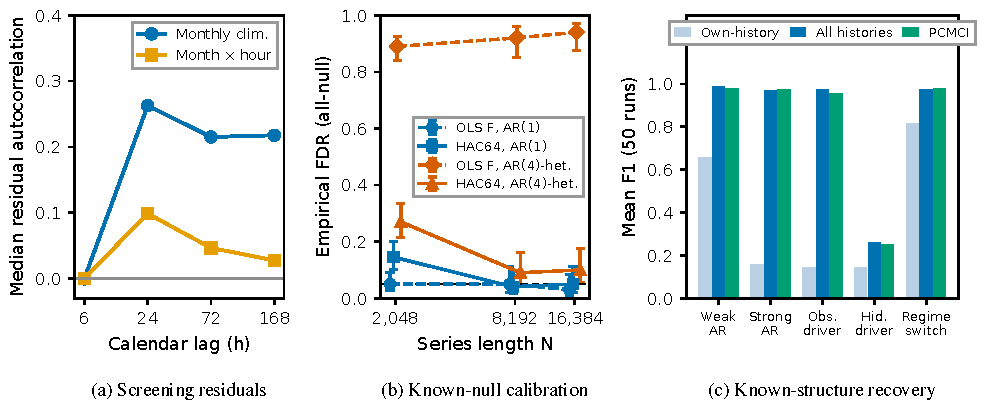
\includegraphics[width=\textwidth]{figures/fig02_calibration.pdf}
\caption{Residual dependence and calibration. Screening residuals are dominated by the diurnal cycle, OLS $F$-tests are badly miscalibrated under autoregressive heteroskedastic nulls whereas HAC inference approaches the nominal level as series lengthen, and own-history screening recovers structure poorly unless the system is weakly coupled.}
\label{fig:calibration}
\end{figure}

The small change in counts does not imply that the $F$-tests were calibrated. In known-null simulations (Figure~\ref{fig:calibration}b), OLS $F$-tests attain the nominal false-discovery rate of 0.05 under autoregressive, homoskedastic noise, but under order-four heteroskedastic noise their empirical FDR is 0.890 at length 2,048 and 0.940 at 16,384, so a longer record does not help. HAC inference reduces the empirical FDR from 0.270 at length 2,048 to 0.100 (95\% interval 0.055--0.174) at 16,384, and from 0.475 to 0.070 when an external calendar mask removes part of the record. The discovery and held-out segments contain 58,437 and 5,884 responses, so HAC-based $q$-values are approximately but not exactly calibrated at our sample sizes. We therefore treat $q<0.05$ as a screening threshold and base our claims on held-out replication.

Known-structure simulations expose a second, more serious problem (Figure~\ref{fig:calibration}c; Table~\ref{tab:benchmark}). Own-history screening recovers every true edge, but with strong autocorrelation its precision is 0.086 and its F1 is 0.158; with an observed common driver its F1 is 0.143, because indirect and common-driver dependencies are predictive given the target's own history alone. Regression on all observed histories restores F1 values of 0.970--0.986 and PCMCI 0.956--0.978. When the common driver is hidden, every method fails (F1 0.252--0.259). These results motivate confirmation under full conditioning and also bound what any method can achieve when relevant drivers are unobserved.

\subsection{Screen, confirm, replicate}
\label{subsec:three_res}

In 1979--2018, the own-history screen retains 2,187 of 2,574 edge--lag hypotheses, and full conditioning confirms 1,550 of them (Table~\ref{tab:threestage}; Figure~\ref{fig:threestage}a). Screening and confirmation disagree on sign for 649 of the 1,550 confirmed hypotheses, so own-history coefficient signs should not be interpreted. In the dense VAR, coefficients at different lags of the same edge alternate in sign for 95.2\% of the 568 confirmed edges with at least two confirmed lags, which indicates that much of the conditional dependence is carried by recent tendencies rather than levels. We therefore interpret magnitudes, replication and predictive gains rather than individual lag signs.

\begin{table}[htbp]
\centering
\caption{Screen, confirm and replicate results by edge type.}
\label{tab:threestage}
\scriptsize
\setlength{\tabcolsep}{3.5pt}
\begin{tabular}{@{}lrrrrrrrrr@{}}
\toprule
& & \multicolumn{2}{c}{1979--2018} & \multicolumn{3}{c}{2019-01-01 to 2023-01-10} & \multicolumn{3}{c}{2023-01-11 to 2025-12-31} \\
\cmidrule(lr){3-4}\cmidrule(lr){5-7}\cmidrule(lr){8-10}
Edge type & Tested & Screened & Confirmed & Replicated & Rate & \shortstack[r]{Control\\rate} & Replicated & Rate & \shortstack[r]{Control\\rate} \\
\midrule
$W\rightarrow H$ & 594 & 502 & 325 & 117 & 0.360 & 0.052 & 101 & 0.311 & 0.059 \\
$H\rightarrow C$ & 594 & 480 & 313 & 133 & 0.425 & 0.100 & 124 & 0.396 & 0.068 \\
$W\rightarrow C$ & 594 & 512 & 311 & 113 & 0.363 & 0.042 & 92 & 0.296 & 0.032 \\
$H\rightarrow H$ & 396 & 342 & 273 & 153 & 0.560 & 0.138 & 142 & 0.520 & 0.130 \\
$T\rightarrow H$ & 198 & 185 & 171 & 137 & 0.801 & 0.296 & 121 & 0.708 & 0.259 \\
$T\rightarrow C$ & 198 & 166 & 157 & 107 & 0.682 & 0.390 & 87 & 0.554 & 0.317 \\
\midrule
\textit{All} & 2,574 & 2,187 & 1,550 & 760 & 0.490 & 0.093 & 667 & 0.430 & 0.078 \\
\bottomrule
\end{tabular}
\end{table}

\begin{figure}[htbp]
\centering
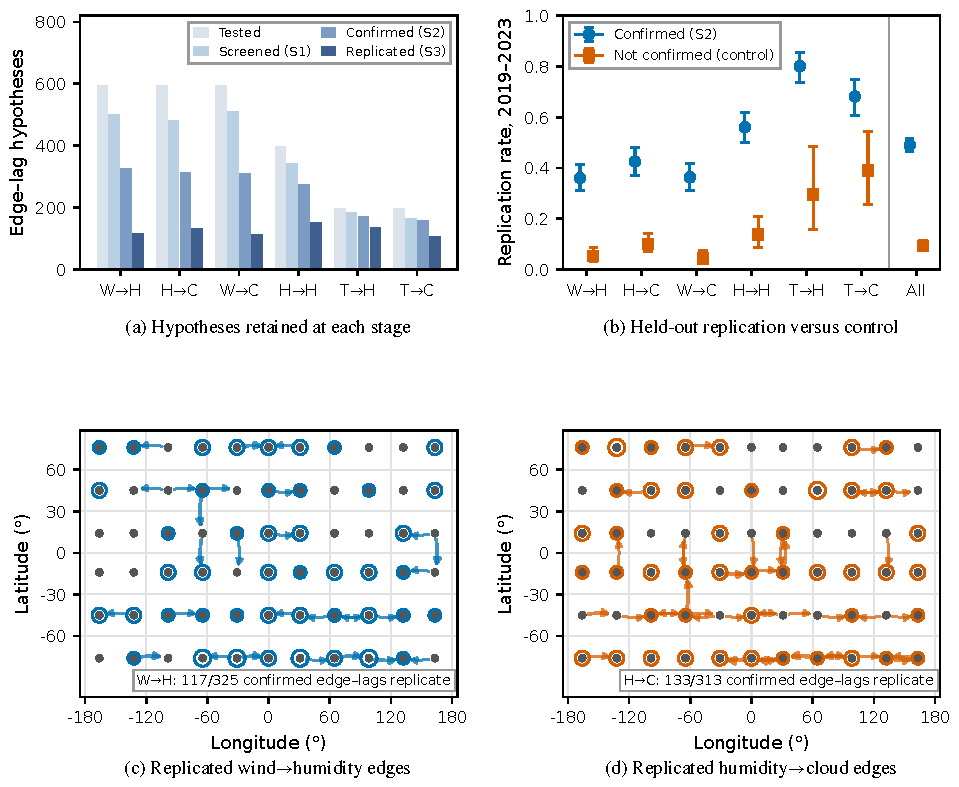
\includegraphics[width=\textwidth]{figures/fig03_three_stage.pdf}
\caption{Screen--confirm--replicate results. Confirmed hypotheses replicate far more often than unconfirmed controls, and replicated cross-region edges are predominantly zonal links between neighbouring regions.}
\label{fig:threestage}
\end{figure}

In the primary held-out segment, 760 of the 1,550 confirmed hypotheses (0.490) replicate with the same sign, compared with 95 of the 1,024 unconfirmed hypotheses (0.093) under the identical rule (Figure~\ref{fig:threestage}b). Of the replicated hypotheses, 416 also improve frozen held-out prediction ($q<0.05$), and 1,363 of the 1,550 confirmed hypotheses (0.879) keep their sign. Replication rates range from 0.360 for wind$\rightarrow$humidity and 0.363 for wind$\rightarrow$cloud to 0.425 for humidity$\rightarrow$cloud, 0.560 for humidity$\rightarrow$humidity and 0.682--0.801 for the local temperature edges. The 760 replicated hypotheses correspond to 450 unique directed edges (of 726 confirmed unique edges); 300 hypotheses link different regions, and 249 of these connect regions in the same latitude row (Figure~\ref{fig:threestage}c,d). Replication is higher for midlatitude (0.531) and polar (0.521) than for tropical targets (0.411). In the second held-out segment, 2023-01-11 to 2025-12-31, 667 confirmed hypotheses (0.430) replicate against 80 of 1,024 controls (0.078), close to the primary segment despite its shorter length.

Replicated dependencies are modest in size. The median absolute coefficient is 0.045 standard deviations for confirmed and 0.080 for replicated hypotheses, the median held-out partial $R^2$ of replicated hypotheses is 0.0029, and their median frozen relative reduction in mean squared error is 0.27\%. Summed over lags, 63\% of replicated humidity$\rightarrow$cloud edges and 90\% of temperature$\rightarrow$humidity edges are positive, whereas wind$\rightarrow$cloud sums are evenly split. The three-stage results are insensitive to removing the diurnal cycle: with a month $\times$ UTC-hour climatology, 2,064 hypotheses are screened, 1,457 confirmed and 721 replicated, against 117 of 1,117 controls (Supplementary Table~S11). By contrast, PCMCI with partial-correlation tests and at most three conditioning variables, applied to all 2,574 hypotheses in 2019--2025, flags 85\% of the strongest screened hypotheses (top quartile of discovery effects), 82\% of the other screened hypotheses and 73\% of the unscreened hypotheses, so at this conditioning budget its agreement does not discriminate between strata.

\subsection{Direction and spatial specificity}
\label{subsec:dir_res}

Under full conditioning, the direction of the humidity--cloud dependence becomes measurable, whereas that of the wind--humidity dependence does not (Table~\ref{tab:direction}; Figure~\ref{fig:direction}a). In 1979--2018, humidity$\rightarrow$cloud has the larger absolute $t$-statistic in 55.2\% of 636 matched pairs (Wilcoxon $p=0.008$), and the asymmetry recurs in both held-out segments (52.2\%, $p=0.049$, in 2019--2023; 53.6\%, $p=0.023$, in 2023--2025), with diurnally adjusted anomalies (55.3\%, $p=0.005$) and with CERES cloud in 2017--2023 (56.3\%, $p=0.014$). Wind$\rightarrow$humidity is not stronger than humidity$\rightarrow$wind (48.4\%, $p=0.14$, in discovery; 48.3\%, $p=0.86$, in 2019--2023), and in 2023--2025 the reverse is marginally stronger (45.8\%, $p=0.024$); wind--cloud pairs are balanced. This contrasts with own-history screening on the same symmetric support, where cloud$\rightarrow$humidity is significant more often than humidity$\rightarrow$cloud (547 versus 508 of 636) and wind$\rightarrow$humidity more often than its reverse (532 versus 475). Orientation inferred from own-history screening is therefore unreliable, and the wind--humidity direction of our pathway is a modelling choice rather than a data-supported finding.

\begin{table}[htbp]
\centering
\caption{Direction tests on the symmetric candidate set under full conditioning.}
\label{tab:direction}
\footnotesize
\setlength{\tabcolsep}{3pt}
\begin{tabular}{@{}p{0.27\textwidth}lll@{}}
\toprule
Measure & $H\rightarrow C$ vs $C\rightarrow H$ & $W\rightarrow H$ vs $H\rightarrow W$ & $W\rightarrow C$ vs $C\rightarrow W$ \\
\midrule
Significant, 1979--2018 & 403 / 375 & 381 / 402 & 378 / 380 \\
Significant, 2019--2023 & 118 / 115 & 91 / 103 & 89 / 88 \\
Significant, 2023--2025 & 107 / 94 & 78 / 77 & 54 / 59 \\
Stronger forward, 1979--2018 & 0.552 (0.008) & 0.484 (0.142) & 0.514 (0.379) \\
Stronger forward, 2019--2023 & 0.522 (0.049) & 0.483 (0.856) & 0.508 (0.402) \\
Stronger forward, 2023--2025 & 0.536 (0.023) & 0.458 (0.024) & 0.472 (0.103) \\
Stronger forward, diurnal, 2019--2023 & 0.553 (0.005) & 0.502 (0.481) & 0.525 (0.466) \\
Stronger forward, CERES, 2017--2023 & 0.563 (0.014) & -- & 0.513 (0.288) \\
Stronger forward, CERES, 2023--2025 & 0.494 (0.708) & -- & 0.519 (0.334) \\
\bottomrule
\end{tabular}
\end{table}

\begin{figure}[htbp]
\centering
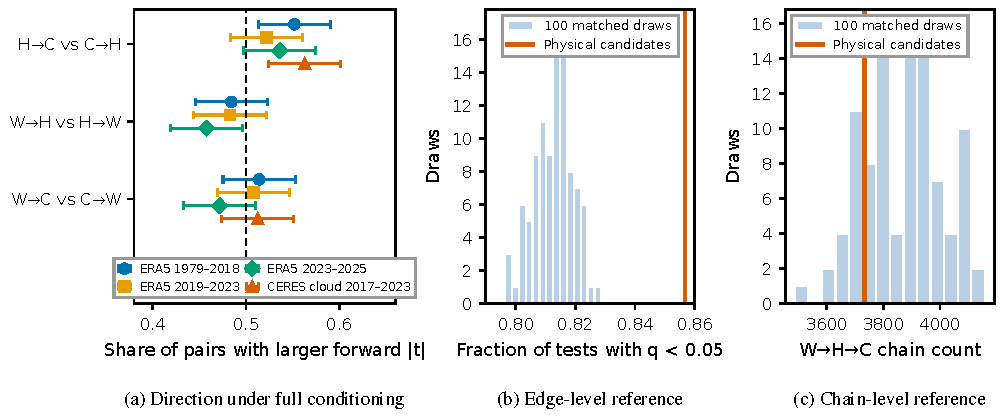
\includegraphics[width=\textwidth]{figures/fig04_direction_nulls.pdf}
\caption{Direction and specificity. Only humidity$\rightarrow$cloud is consistently stronger than its reverse; physics-guided edges are significant more often than all 100 distance-matched random candidate sets, but their chain count lies inside the null distribution.}
\label{fig:direction}
\end{figure}

The physics-guided candidates carry modest edge-level specificity beyond spatial background (Figure~\ref{fig:direction}b). In the full-record screen with HAC inference and global BH, 0.857 of the 2,574 hypotheses are significant, compared with a mean of 0.813 (2.5--97.5\% range 0.799--0.823) across 100 distance-matched random candidate sets, which the observed rate exceeds in every draw. The excess holds for wind$\rightarrow$humidity (0.857 versus 0.797), humidity$\rightarrow$cloud (0.808 versus 0.760) and wind$\rightarrow$cloud (0.874 versus 0.808). Chain abundance, by contrast, is not enriched: the physical graph contains 3,733 lag-resolved wind--humidity--cloud chains against a null mean of 3,871 (range 3,635--4,101; upper-tail probability 0.81), and on the symmetric support 4,249 against 4,288 (0.57). Chains that close a triad, in which wind also connects directly to the cloud target, are 1.60 times more frequent than in the null graphs (424 versus 264), which we attribute to spatial coherence among adjacent regions rather than to mediation.

\subsection{Regime and seasonal dependence}
\label{subsec:regime_res}

The descriptive full-record screen is nearly saturated in every regime (Table~\ref{tab:regime}). High-humidity and high-cloud regimes contain about one fifth of the responses and correspondingly fewer significant tests, and the shares of wind$\rightarrow$humidity, humidity$\rightarrow$cloud and cross-region edges vary by less than 0.04 across regimes. Because these regime graphs are selected separately, and the humidity and cloud masks condition on the response, their differences, including those in chain counts and Jaccard distances (Supplementary Table~S6), are not evidence of state dependence.

\begin{table}[htbp]
\centering
\caption{Descriptive full-record screening across regimes.}
\label{tab:regime}
\footnotesize
\setlength{\tabcolsep}{4pt}
\begin{tabular}{@{}lrrrrrrr@{}}
\toprule
& & & \multicolumn{2}{c}{Significant tests} & \multicolumn{3}{c}{Share of HAC-significant tests} \\
\cmidrule(lr){4-5}\cmidrule(lr){6-8}
Regime & Responses & Tests & OLS $F$ & HAC64 & $W\rightarrow H$ & $H\rightarrow C$ & Cross-region \\
\midrule
All & 68,665 & 2,574 & 2,233 & 2,206 & 0.231 & 0.218 & 0.599 \\
DJF & 16,965 & 2,574 & 2,010 & 1,962 & 0.243 & 0.214 & 0.584 \\
JJA & 17,296 & 2,574 & 2,026 & 2,001 & 0.218 & 0.220 & 0.589 \\
High humidity & 13,731 & 2,574 & 1,863 & 1,790 & 0.230 & 0.211 & 0.573 \\
Normal humidity & 41,200 & 2,574 & 2,144 & 2,104 & 0.232 & 0.220 & 0.588 \\
High cloud & 13,734 & 2,574 & 1,849 & 1,776 & 0.239 & 0.206 & 0.565 \\
Normal cloud & 54,931 & 2,574 & 2,183 & 2,156 & 0.231 & 0.218 & 0.596 \\
\midrule
Total & -- & 18,018 & 14,308 & 13,995 & -- & -- & -- \\
\bottomrule
\end{tabular}
\end{table}

Direct interaction tests separate state dependence from selection (Figure~\ref{fig:regimes}c). Source-by-cloud-state interactions pass BH in 173 of 2,574 tests in 1979--2018 when the state is concurrent and in 124 when it is defined 24~h earlier, but in only 4 and 1 of the 2,574 held-out tests. Humidity-state interactions fall from 117 and 107 discovery tests to 36 and 37 held-out tests. External states defined from the antecedent Ni\~no-3.4 anomaly give small slope contrasts whose signs change in 30 of 108 high-minus-middle and 24 of 108 low-minus-middle comparisons once the six physical controls are added (Supplementary Table~S7). We therefore find no replicable modulation of the dependencies by cloud or ENSO state at this design, and only weak modulation by the humidity state.

\begin{figure}[htbp]
\centering
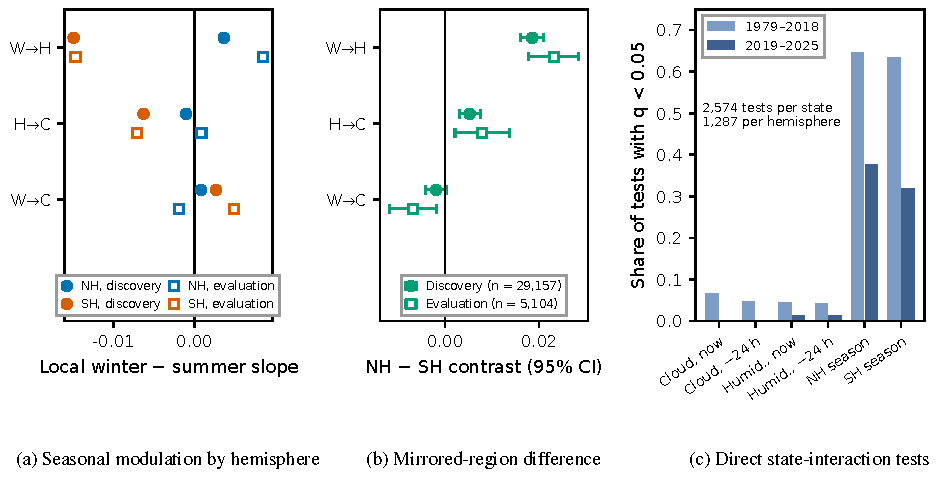
\includegraphics[width=\textwidth]{figures/fig05_regimes.pdf}
\caption{Seasonal and state dependence. Seasonal modulation of wind$\rightarrow$humidity has opposite signs in the two hemispheres, and cloud-state interactions found in 1979--2018 do not replicate in 2019--2025.}
\label{fig:regimes}
\end{figure}

Seasonal modulation, in contrast, is pervasive and replicates: local winter-minus-summer slope differences pass BH in 830 and 816 of 1,287 discovery tests in the NH and SH and in 485 and 411 held-out tests. Its sign, however, differs between hemispheres (Figure~\ref{fig:regimes}a). For wind$\rightarrow$humidity, the mean signed winter-minus-summer slope is $+0.0036$ in the NH and $-0.0149$ in the SH in 1979--2018 ($+0.0084$ and $-0.0147$ in 2019--2025), and the mirrored-region contrast $\Delta_{\mathrm{NH}}-\Delta_{\mathrm{SH}}$ is $0.0185$ (95\% interval $0.0160$--$0.0210$) in discovery and $0.0231$ ($0.0178$--$0.0284$) held out (Figure~\ref{fig:regimes}b). Humidity$\rightarrow$cloud shows a smaller contrast ($0.0053$ and $0.0079$), and wind$\rightarrow$cloud none in discovery ($-0.0019$, $-0.0040$ to $0.0003$) and a small negative one held out ($-0.0068$, $-0.0118$ to $-0.0017$). A globally pooled DJF regime therefore mixes NH winter with SH summer, and the dependencies do not strengthen uniformly in winter.

\subsection{Pathway timing, mediation and moisture transport}
\label{subsec:timing_res}

Summed path lags are properties of the search window rather than transit times. The screened all-regime graph contains 3,777 chains with a mean summed lag of 3.99 steps (23.9~h), almost exactly the four steps expected under uniform detection over three lags, and extending the window to twelve lags moves the mean single-edge lag to 6.1--6.3 steps, close to the uniform value of 6.5 (Supplementary Table~S10). In joint models, the absolute-coefficient centroid tracks the uniform reference $(L+1)/2$ for $L=3$, 6 and 12 (2.01, 3.57 and 6.44 steps; Figure~\ref{fig:timing}a), and in simulations with a single true lag of two steps the centroid still drifts from 2.00 to 3.88 as the window widens, although the peak lag is recovered in all 100 replicates. Held-out information is not confined to short lags either: deleting source lags 1--3, 4--8 or 9--12 increases held-out error in 33, 28 and 30 of 36 pairs (median $\Delta R^2=6.5\times10^{-4}$, $9.7\times10^{-4}$ and $4.0\times10^{-4}$; Figure~\ref{fig:timing}b), and each window carries information in both held-out segments, so the data do not identify a dominant transit time.

\begin{figure}[htbp]
\centering
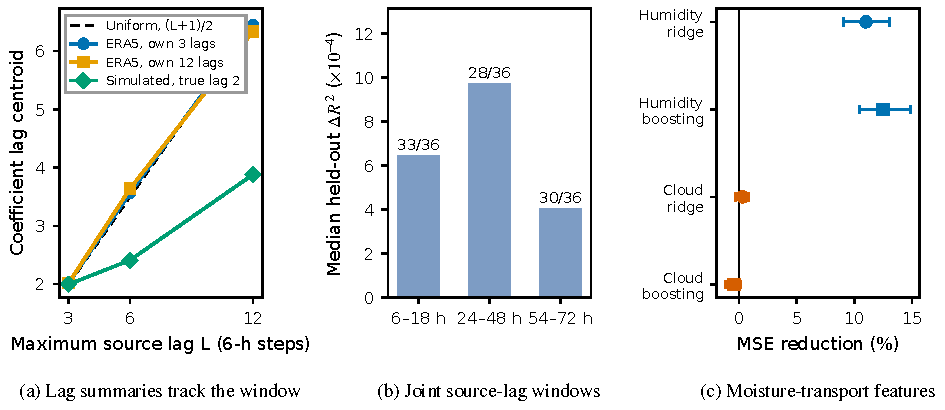
\includegraphics[width=\textwidth]{figures/fig06_timing_transport.pdf}
\caption{Timing and transport. Lag summaries follow the tested window even when the true lag is short, held-out information is spread over all three lag windows, and moisture-transport features improve humidity but not cloud prediction.}
\label{fig:timing}
\end{figure}

Time-aligned path models show that humidity explains only part of the wind--cloud dependence. Among the 20 strong paths, the humidity$\rightarrow$cloud stage given wind improves held-out prediction in 19 (median $\Delta R^2=1.6\times10^{-3}$), the wind$\rightarrow$humidity stage in 20 ($5.2\times10^{-4}$) and the direct wind$\rightarrow$cloud term given the specified intermediate humidity still in 14 ($1.7\times10^{-4}$). With the six physical controls taken before the path source, these counts are 17, 19 and 14 and the median gains shrink to $5.3\times10^{-4}$, $1.0\times10^{-4}$ and $6.1\times10^{-5}$. The earlier mean attenuation of 3.69\% after adding target-region humidity is therefore a coarse summary of a partial, control-sensitive dependence and not an identified mediated fraction (Supplementary Tables~S10 and~S12). Projecting wind and moisture flux onto the source--target direction adds held-out information in 331 and 320 of 396 models, but with small median gains ($\Delta R^2=4.6\times10^{-5}$ and $7.9\times10^{-5}$). In the two Atlantic footprints, transport features reduce the held-out mean squared error of the 6-h humidity change by 11.02\% (95\% interval 9.09--13.10\%) for ridge regression and 12.51\% (10.42--14.87\%) for gradient boosting, whereas the cloud-cover changes are 0.32\% ($-0.30$ to $0.79$\%) and $-0.44$\% ($-1.14$ to $0.16$\%) (Figure~\ref{fig:timing}c). Resolved horizontal transport thus carries information about subsequent humidity, but not enough about cloud, which also depends on vertical motion, stability and microphysics.

\subsection{Independent satellite cloud}
\label{subsec:ceres_res}

ERA5 and CERES cloud anomalies agree moderately (Figure~\ref{fig:ceres}a). Over 2017-01-01 to 2023-01-10, the median correlation is 0.758 at the grid scale and 0.763 at the regional scale (range 0.371--0.914), with weakest agreement in polar regions (Supplementary Table~S15); CERES cloud cover is 4.0 percentage points higher on an area-weighted basis. Agreement is the same in 2023-01-11 to 2025-12-31 (0.764 and 0.778), whereas fields requested on the coarse CDS grid had lowered the grid-scale correlation in this segment to 0.612, independent evidence that the regridding route matters.

\begin{figure}[htbp]
\centering
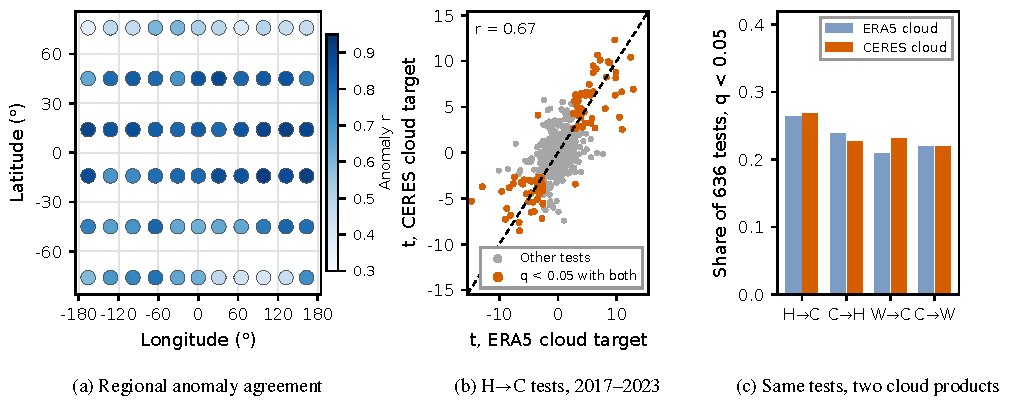
\includegraphics[width=\textwidth]{figures/fig07_ceres.pdf}
\caption{Satellite cloud substitution. Regional ERA5 and CERES cloud anomalies agree moderately, and humidity$\rightarrow$cloud tests give similar prevalence and consistent signs with either cloud product.}
\label{fig:ceres}
\end{figure}

Replacing ERA5 cloud by CERES cloud leaves the humidity--cloud dependence intact (Table~\ref{tab:ceres}; Figure~\ref{fig:ceres}b,c). Under full conditioning in 2017--2023, 168 humidity$\rightarrow$cloud tests are significant with ERA5 cloud and 171 with CERES cloud; 94 are significant with both, 92 of them with the same sign, and the $t$-statistics correlate at 0.67 across all 636 tests. Results are similar for the reverse direction and for wind--cloud pairs, with lower $t$-correlations for the latter (0.46--0.51), and they are unchanged with a month $\times$ UTC-hour climatology. The humidity$\rightarrow$cloud dependence is therefore not an artefact of the reanalysis cloud scheme, and it recurs in 2023-01-11 to 2025-12-31, where 109 and 88 tests are significant with ERA5 and CERES cloud and all 51 tests significant with both share the sign ($t$-correlation 0.66). The direction asymmetry, however, is not detected with CERES cloud in this shorter segment (49.4\% of pairs, $p=0.71$, against 53.9\%, $p=0.023$, with ERA5 cloud; Table~\ref{tab:direction}), so the satellite support for the humidity$\rightarrow$cloud orientation rests on 2017--2023.

\begin{table}[htbp]
\centering
\caption{Tests with ERA5 and CERES cloud, 2017-01-01 to 2023-01-10.}
\label{tab:ceres}
\footnotesize
\setlength{\tabcolsep}{2.8pt}
\begin{tabular}{@{}lllrrrl@{}}
\toprule
& Own history & \multicolumn{4}{c}{Full conditioning} & Diurnal \\
\cmidrule(lr){2-2}\cmidrule(lr){3-6}\cmidrule(lr){7-7}
Edge type & ERA5 / CERES & ERA5 / CERES & Both & Same sign & $t$ corr. & ERA5 / CERES \\
\midrule
$H\rightarrow C$ & 378 / 396 & 168 / 171 & 94 & 92 & 0.67 & 157 / 155 \\
$C\rightarrow H$ & 412 / 435 & 152 / 144 & 84 & 84 & 0.73 & 138 / 131 \\
$W\rightarrow C$ & 383 / 388 & 133 / 147 & 56 & 50 & 0.46 & 129 / 140 \\
$C\rightarrow W$ & 373 / 385 & 139 / 139 & 54 & 53 & 0.51 & 120 / 123 \\
\bottomrule
\end{tabular}
\end{table}

\subsection{Wind--humidity eddy convergence}
\label{subsec:whec_res}

The pre-specified test supports a WHEC effect on cloud (Figure~\ref{fig:whec}). In midlatitude regions, the frozen WHEC block reduces the held-out cloud-prediction error by 0.456\% in 2019--2023 (HAC $z=10.6$) and by 0.359\% in 2023--2025 ($z=6.8$), against 0.149\% and 0.144\% in the tropics; the midlatitude excess of 0.307 and 0.215 percentage points ($z=6.6$ and 3.8) satisfies E2. The remote-region and placebo versions give midlatitude error reductions between $-0.016$\% and $-0.001$\% ($z$ from $-2.2$ to $-0.2$), so both controls fail E1, and the frozen decision rule classifies the effect as supported in both held-out segments. The effect is not confined to the midlatitudes: polar regions gain 0.501\% and 0.623\%, as much as or more than midlatitude regions. All 22 midlatitude regions gain in 2019--2023 and 20 in 2023--2025.

\begin{figure}[htbp]
\centering
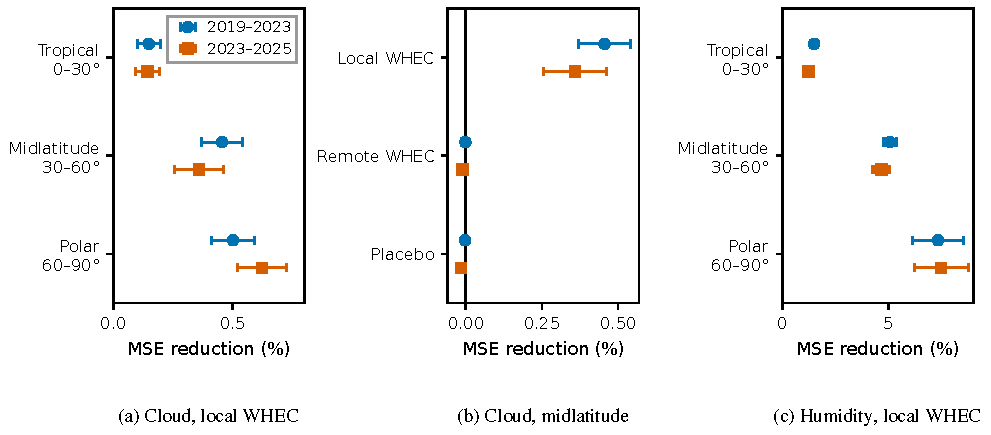
\includegraphics[width=\textwidth]{figures/fig08_whec.pdf}
\caption{Wind--humidity eddy convergence test. Frozen 1979--2018 gains in held-out cloud (a) and humidity (c) prediction by latitude band, and midlatitude cloud gains of the local index and its two controls (b), with 95\% HAC intervals.}
\label{fig:whec}
\end{figure}

Lag-specific tests agree (Table~\ref{tab:whec}). Of the 198 local cloud hypotheses, 168 pass the screen and 139 are confirmed, against one in each control family; 86 replicate in 2019--2023 and 66 in 2023--2025, whereas 1 of 59 unconfirmed local hypotheses does so in each segment. All 54 confirmed coefficients at 6~h are positive and 39 of the 44 at 12~h are negative, so cloud follows a recent increase in eddy convergence rather than its level. For humidity, the secondary target, the WHEC block reduces the midlatitude error by 5.07\% and 4.66\%, 3.4 and 3.8 times the tropical gain, as expected from the moisture budget. With CERES cloud as both predictor and outcome in refits on 2017--2023 and 2023--2025, 64 and 41 of the 198 local cloud hypotheses keep their discovery sign at $q<0.05$, against at most 6 for the control families, although midlatitude support with CERES cloud is weak in the shorter second segment (6 of 66). The gains are small: a reduction of about 0.4\% in the cloud-prediction error matches the non-significant cloud change in the two-footprint transport experiment and becomes detectable only when 22 regions are pooled.

\begin{table}[htbp]
\centering
\caption{Wind--humidity eddy convergence test, 198 lag-specific hypotheses per family and target; families use the local WHEC, the WHEC of a remote region in the same latitude band, or the time-shifted placebo. Replicated: confirmed and same-sign replication $q<0.05$; unconfirmed: the same rule applied to hypotheses that failed Stage~1 or~2; CERES: discovery sign and $q<0.05$ in refits with CERES cloud.}
\label{tab:whec}
\scriptsize
\setlength{\tabcolsep}{3.5pt}
\begin{tabular}{@{}llrrrrrrrr@{}}
\toprule
& & & & \multicolumn{2}{c}{Replicated} & \multicolumn{2}{c}{Unconfirmed} & \multicolumn{2}{c}{CERES} \\
\cmidrule(lr){5-6}\cmidrule(lr){7-8}\cmidrule(lr){9-10}
Family & Target & Screened & Confirmed & 2019--23 & 2023--25 & 2019--23 & 2023--25 & 2017--23 & 2023--25 \\
\midrule
Local & Cloud & 168 & 139 & 86 & 66 & 1 & 1 & 64 & 41 \\
 & Humidity & 189 & 178 & 139 & 141 & 2 & 3 & -- & -- \\
Remote & Cloud & 47 & 1 & 0 & 0 & 0 & 2 & 0 & 0 \\
 & Humidity & 21 & 1 & 0 & 0 & 0 & 0 & -- & -- \\
Placebo & Cloud & 1 & 1 & 0 & 1 & 0 & 0 & 6 & 0 \\
 & Humidity & 1 & 0 & -- & -- & 0 & 0 & -- & -- \\
\bottomrule
\end{tabular}
\end{table}

\subsection{Comparison with existing methods}
\label{subsec:bench_res}

Table~\ref{tab:benchmark} summarizes the benchmarks. In the known-structure systems, all-history regression and PCMCI are comparably accurate and both far exceed own-history regression, while HAC inference lowers F1 by at most 0.02 relative to OLS (Supplementary Table~S13). In the regime-switching benchmark, hidden-state Regime-PCMCI raises F1 from 0.610 for pooled PCMCI to 0.826 and recovers the state sequence with mean accuracy 0.846, but it is variable across replicates (standard deviation 0.237) and about 750 times slower; methods given the true state masks reach 0.936--0.983. Regime-PCMCI therefore provides a capability that our prescribed regimes do not, namely learning unknown states. In lattice benchmarks, CaStLe reaches F1 of 0.971--0.976 when spatial structure is homogeneous but drops to 0.780--0.786, with precision of about 0.65, when it is heterogeneous, where local estimators retain precision above 0.95. Neither benchmark makes Causal WeatherGraph a more accurate identification algorithm; its contribution is the verification layer of confirmation, replication and negative controls, which these methods do not provide.

\begin{table}[htbp]
\centering
\caption{Benchmarks with known structure. Panel A: mean F1 over 50 replicates and runtime per fit; Panel B: regime-switching system, 20 replicates; Panel C: lattice systems, mean F1 over 25 replicates.}
\label{tab:benchmark}
\footnotesize
\setlength{\tabcolsep}{3.5pt}
\begin{tabular}{@{}lrrrrrr@{}}
\toprule
\multicolumn{7}{@{}l}{\textit{A. Six-variable systems}} \\
Method & \shortstack[r]{Weak\\AR} & \shortstack[r]{Strong\\AR} & \shortstack[r]{Observed\\driver} & \shortstack[r]{Hidden\\driver} & \shortstack[r]{Regime\\switch} & s/fit \\
\midrule
Own-history OLS & 0.654 & 0.158 & 0.143 & 0.143 & 0.816 & 0.07 \\
Own-history HAC & 0.639 & 0.157 & 0.142 & 0.142 & 0.801 & 0.07 \\
All-history OLS & 0.986 & 0.970 & 0.974 & 0.259 & 0.976 & 0.22 \\
All-history HAC & 0.976 & 0.966 & 0.965 & 0.258 & 0.957 & 0.22 \\
PCMCI & 0.978 & 0.973 & 0.956 & 0.252 & 0.976 & 0.48 \\
\bottomrule
\end{tabular}

\vspace{6pt}
\begin{tabular}{@{}llrrlrr@{}}
\toprule
\multicolumn{7}{@{}l}{\textit{B. Regime-switching system}} \\
Method & Given & Precision & Recall & F1 (SD) & s/fit & Peak MiB \\
\midrule
Pooled PCMCI & none & 0.473 & 0.871 & 0.610 (0.040) & 0.24 & 181 \\
Regime-PCMCI & state count & 0.859 & 0.871 & 0.826 (0.237) & 179.66 & 862 \\
Own-history OLS & true masks & 0.889 & 0.996 & 0.936 (0.047) & 0.10 & 181 \\
All-history HAC & true masks & 0.893 & 0.996 & 0.936 (0.065) & 0.19 & 182 \\
All-history OLS & true masks & 0.966 & 0.996 & 0.978 (0.035) & 0.19 & 182 \\
PCMCI & true masks & 0.973 & 0.996 & 0.983 (0.025) & 0.31 & 182 \\
\bottomrule
\end{tabular}

\vspace{6pt}
\begin{tabular}{@{}lrrrr@{}}
\toprule
\multicolumn{5}{@{}l}{\textit{C. Lattice systems}} \\
& \multicolumn{2}{c}{Homogeneous} & \multicolumn{2}{c}{Heterogeneous} \\
\cmidrule(lr){2-3}\cmidrule(lr){4-5}
Method & $6\times6$ & $10\times10$ & $6\times6$ & $10\times10$ \\
\midrule
CaStLe (official) & 0.971 & 0.976 & 0.780 & 0.786 \\
Local own-history OLS & 0.764 & 0.758 & 0.720 & 0.757 \\
Local multivariable OLS & 0.724 & 0.717 & 0.680 & 0.727 \\
Local PCMCI & 0.739 & 0.735 & 0.698 & 0.736 \\
\bottomrule
\end{tabular}
\end{table}

The framework scales to the full problem on a workstation (Intel Core Ultra 9 275HX, 64~GB memory). Screening the 18,018 regime tests takes 157~s, fitting and testing the dense VAR(3) on 58,437 discovery responses with 264 outcomes takes 29~s, and the complete three-stage analysis over both candidate sets and all segments takes 118~s with a peak memory of 2.4~GB.

\subsection{Robustness of the screening stage}
\label{subsec:robust_res}

The screening stage is stable under perturbation, but this stability mainly reflects its saturation. With $k=2$, 857 of 858 candidates are significant at some lag; expanding the neighbourhood to $k=4$, 6 and 8 recovers all 857 edges, different preprocessing choices preserve 85--88\% of lag-resolved chains, and alternative regionalizations and historical periods give similar significance rates (Supplementary Tables~S2--S5). Bootstrap resampling of the lagged calendar design with block lengths of 64, 128 and 256 steps gives nearly identical coefficient intervals across block lengths for twelve fixed edge--regime models (Supplementary Table~S8). These analyses show that the screened graph is reproducible, not that its structure is specific; specificity and replication are assessed in Sections~\ref{subsec:three_res} and~\ref{subsec:dir_res}.

\section{Discussion and Limitations}
\label{sec:discussion}

\subsection{What replicates and what does not}

The three stages answer different questions. Screening asks whether a source lag adds information beyond the target's own history, which is true of almost every physically motivated candidate in a strongly coupled reanalysis. Confirmation asks whether the information survives conditioning on all other observed histories, which removes 29\% of the screened hypotheses and reverses the sign of many others. Replication asks whether confirmed dependencies recur in years not used for any modelling decision, which roughly half of them do in 2019--2023, about five times as often as unconfirmed hypotheses under the same rule, and 43\% do in 2023--2025. The replicated set of 760 conditional dependencies, which is concentrated at mid and high latitudes and in zonally adjacent regions and whose held-out information is not confined to the shortest lags, is the principal empirical output of our framework.

Several properties that a screening-based description of the pathway suggests do not survive. Chain counts are not enriched relative to distance-matched random candidates, so the abundance of wind--humidity--cloud chains reflects the density of a spatially coherent background. The wind$\rightarrow$humidity orientation is imposed by the candidate list rather than supported by the data. The mean summed lag of about 24~h is fixed by the search window. A globally pooled DJF regime mixes opposite local seasons, and cloud-state differences found in the discovery period do not replicate. Humidity remains a partial and control-sensitive channel for wind--cloud dependence rather than an identified mediator.

\subsection{Physical interpretation}

The most robust directional result, a modest asymmetry favouring humidity$\rightarrow$cloud over cloud$\rightarrow$humidity under full conditioning, is consistent with the role of moisture as a cloud-controlling factor \citep{Andersen2023CloudSensitivities}; that it persists with satellite cloud argues against an artefact of the reanalysis cloud scheme. The symmetric wind--humidity dependence is consistent with both variables responding to the same synoptic systems: scalar wind speed measures circulation intensity rather than transport, and only the projected moisture flux carries directional transport information, which adds little beyond scalar wind at the regional scale. The hemispheric difference in seasonal modulation plausibly reflects hemispheric differences in storm tracks, which depend on topography and ocean energy transport \citep{Shaw2022Stormier} and which a global DJF average conflates. The eddy-convergence result qualifies the transport picture. The covariance of wind and humidity anomalies, which no linear model of regional anomalies represents, carries information about cloud six hours later beyond the dense autoregression and the linear transport terms, and more outside the tropics than inside them. This pattern is consistent with the link between extratropical cloud water and moisture convergence \citep{McCoy2022Extratropical} and with cloud formation in the ascending moist airstreams of cyclones \citep{Heitmann2024WCB}, and the positive coefficient at 6~h followed by a negative one at 12~h indicates a response to a recent increase in eddy moisture import. The cloud gains nonetheless remain small, and both the transport experiment and the eddy index show that horizontal moisture transport at 850~hPa explains little of the cloud variability, which also depends on vertical motion, stability and microphysics \citep{WilsonKemsley2024HighCloud}.

\subsection{Implications for information sciences}

Three lessons apply beyond the atmosphere. First, single-stage screening with own-history controls is a recall device, not a discovery procedure: in strongly coupled systems it reports indirect and common-driver dependencies with high confidence, and their signs are unreliable. Second, verification of a discovered graph requires information the discovery did not use: held-out periods with frozen procedures and a negative-control family make replication rates interpretable, whereas high overlap among nearly saturated graphs does not. Third, data provenance is part of the inference: a change of acquisition route within the record altered the noise level, the agreement with an independent product and even the apparent direction of a dependence. These design elements, namely domain-constrained candidates, full conditioning, held-out replication with negative controls and provenance checks, transfer to other large spatio-temporal records such as traffic, energy, hydrological and epidemiological surveillance data.

\subsection{Limitations and future directions}

Our conclusions are bounded in five ways. First, all real-data results are conditional linear predictive dependencies in an observational reanalysis; the hidden-driver simulations show that no method we tested recovers structure when relevant drivers are unobserved, and the six physical controls do not form a complete adjustment set. Second, HAC-based $q$-values are only approximately calibrated at our sample sizes, so stage counts should be read as screening statistics, while replication rates and negative controls carry the inferential weight. Third, the held-out years also enter the descriptive full-record screening; preprocessing, selection and coefficients were frozen before replication, and the eddy-convergence test was frozen before any of its results, but these years had been examined in other analyses, so a prospective test on future data would be stronger. Fourth, regional aggregation, a single pressure level and scalar wind speed simplify vertical structure and transport direction, and the 850-hPa level is below ground in some cells; the eddy index is a resolved-scale, single-level horizontal term that omits vertical and subgrid transport. Fifth, the satellite comparison covers 2017--2025 and total cloud only, and its support for the humidity$\rightarrow$cloud orientation rests on 2017--2023. Future work can extend the confirmation stage to nonlinear and regime-learning estimators, integrate vertically resolved moisture budgets, and test the replicated set prospectively as new reanalysis years become available.

\section{Conclusion}
\label{sec:conclusion}

We introduced Causal WeatherGraph, a screen--confirm--replicate framework for discovering lagged dependencies in large spatio-temporal records, and applied it to wind, humidity and cloud in 47 years of global reanalysis. Known-null and known-structure simulations showed that a single-stage own-history screen recovers true edges but cannot separate them from indirect and common-driver dependencies, and that conditioning on all observed histories followed by held-out replication separates replicable dependencies from shared-history, indirect and spatial-background artefacts. Of 2,574 physics-guided edge--lag hypotheses, 1,550 were confirmed under full conditioning and 760 replicated in 2019--2023, five times the rate of unconfirmed controls, with a similar rate in a second held-out period, 2023--2025. The replicated dependencies are small, are organized zonally at mid and high latitudes, and, in the pairs examined, carry held-out information at lags from 6 to 72~h rather than at a single transit time. Humidity$\rightarrow$cloud is modestly stronger than its reverse in both held-out periods and, in 2017--2023, with satellite cloud, whereas the wind--humidity direction, chain enrichment, a fixed 24-h transit time, uniform winter strengthening and cloud-state regimes are not supported. A pre-specified wind--humidity eddy convergence, the quadratic part of an exact decomposition of the moisture flux, adds small but replicated held-out information about cloud, 2.5--3.1 times more in the midlatitudes than in the tropics and comparably at high latitudes, whereas remote-region and time-shifted versions add none. The appropriate conclusion is therefore not that we have identified an interventional wind--humidity--cloud chain, but that we have isolated a replicable set of conditional lagged dependencies and a procedure that makes such claims verifiable.

\section*{Data and code availability}

The analysis code, configurations and summary tables are available at \url{https://github.com/gengx-prog/causal-weathergraph}; the revision analyses are in the \texttt{revision/} directory of that repository, including the eddy-convergence index and test (\texttt{make\_whec\_index.py}, \texttt{run\_whec\_test.py}), whose frozen design file and its SHA-256 hash are part of the Supplementary Data. Machine-readable edge-level results for all screening, confirmation and replication tests, including region identifiers, variables, lags, coefficients, standard errors, $p$- and $q$-values, partial $R^2$ and held-out statistics, are provided as Supplementary Data. ERA5 data are available from the Copernicus Climate Data Store, the WeatherBench~2 ERA5 product from its public archive, CERES SYN1deg Edition~4.2 data from the NASA Langley Atmospheric Science Data Center, and the Ni\~no-3.4 index from the NOAA Physical Sciences Laboratory.

\section*{Declaration of competing interest}

The author declares no competing financial interests or personal relationships that could have influenced the work reported in this paper, and is not a member of the editorial board of this journal.

\section*{Declaration of generative AI and AI-assisted technologies in the writing process}

During the preparation and revision of this manuscript, the author used Claude (Anthropic) for language editing, code review, analysis scripting and figure preparation, and OpenAI Codex for code development and the execution of revision analyses. The author reviewed and edited all generated text and code, verified the analyses and references, and takes full responsibility for the content of the publication.

\bibliographystyle{elsarticle-num}
\bibliography{Causal_WeatherGraph_references}

\end{document}
